% ----------------------------------------------------------------------
%                   LATEX TEMPLATE FOR PhD THESIS
% ----------------------------------------------------------------------

% based on Harish Bhanderi's PhD/MPhil template, then Uni Cambridge
% http://www-h.eng.cam.ac.uk/help/tpl/textprocessing/ThesisStyle/
% corrected and extended in 2007 by Jakob Suckale, then MPI-CBG PhD programme
% and made available through OpenWetWare.org - the free biology wiki
% and finally modified in 2015-2017 by Holger Nahrstaedt
% https://github.com/holgern/TUB_PhDThesisTemplate

%: Style file for Latex
% Most style definitions are in the external file PhDthesisTUB.
% In this template package, it can be found in ./Classes/

\documentclass[twoside,11pt,online,a4paper,pdfa1,custommargin,numbered,biblatex]{Classes/PhDthesisTUB}
% *********************** Choosing pdfx standard ******************************
% `pdfa1'
% `pdfa2'
% `pdfx3'
% *********************** Change Thesis-Language to German ******************************
% default is english
% `german' : language is set to german
%
% % *********************** Choosing oneside / twoside ******************************
% `oneside' : layout is optimized for one-side print
% `twoside' : layout is optimized for two-side print
% *********************** Choosing print / online ******************************
% `print' : pdf-file is optimized for print
% `online' : pdf-file is optimized for online submission. The links are colorfull.
% *********************** Choosing biblatex or bibtex ******************
% `biblatex' : biblatex is used. Biblatex is automatically set when using xetex
%
% *********************** Choosing bibliographystyle ******************
% `numbered' : (default option) e.g. [1], [2]
% `authoryear' :  e.g. Name (2008)
% `custombib' : Use your own style, which is defined in preamble.tex
% *********************** Choosing the Fonts size ******************
% `9pt'
% `10pt'
% `11pt'
% `12pt'
% *********************** Choosing the paper size ******************
% `letterpaper'
% `a4paper'
% `a5paper'
% *********************** Choosing the Fonts in Class Options when using pdflatex ******************
% 
%  On Windows, the packge cm-super has to be installed!
%
% `' :  computer modern
% `fontA' :  newtxmath
% `fontB' :  cmbright
% `fontC' :  libertine,newtxmath
% `fontD' :  concmath
% `fontE' :  iwona
% `fontF' :  kurier	
% `fontG' :  anttor
% `fontH' :  kmath,kerkis
% `fontI' :   mathdesign (Utopia)
% `fontJ' :  fouriernc
% `fontK' :  pxfonts
% `fontL' :  mathpazo
% `fontM' :  mathpple
% `fontN' :  txfonts
% `fontO' :  mathtime (Belleek)
% `fontP' :  mathptmx	times	
% `fontQ' :  mbtimes	omega
% `fontR' :  arev
% `fontS' :  mathdesign (Charter)	
% `fontT' :  comicsans
% `fontU' :  mathdesign (Garamond)
% `fontV' :  fourier	utopia
% `fontW' :  ccfonts,eulervm
%
% `customfont': Use `customfont' option in the document class and load the
% package in the preamble.tex
%
% default or leave empty: `Latin Modern' font will be loaded.
%
% *********************** Choosing the Fonts in Class Options when using xelatex/lualatex ***********
%
% `' :  computer modern
% `fontA' :  XITS - XITS Math
% `fontB': Cambria - Cambria Math
% 'fontC': Libertinus - Libertinus Math
% 'fontD': TeX Gyre Pagella - Asana Math
% 'fontE': TeX Gyre Pagella - TeX Gyre Pagella Math
% 'fontF': TeX Gyre Schola - TeX Gyre Schola Math
% 'fontG': TeX Gyre Termes - TeX Gyre Termes Math
% 'fontH': TeX Gyre Bonum - TeX Gyre Bonum Math
% 'fontI': DejaVu Sans - TeX Gyre DejaVu Math
%
% `customfont': Use `customfont' option in the document class and load the
% package in the preamble.tex
%
% default or leave empty: `Latin Modern' font will be loaded.
%
% ************************* Custom Page Margins ********************************
%
% `custommargin`: Use `custommargin' in options to activate custom page margins,
% which can be defined in the preamble.tex. Custom margin will override
% print/online margin setup.
%
% ************************* other options ********************************
% `abstract`: Only the title-page and the abstracts are generated
%

% -*- root: ../thesis.tex -*-
%!TEX root = ../thesis.tex
% ******************************************************************************
% ****************************** Custom Margin *********************************
% Add `custommargin' in the document class options to use this section
% Set {innerside margin / outerside margin / topmargin / bottom margin}  and
% other page dimensions
\ifCLASSINFOcustommargin
  %\RequirePackage[left=37mm,right=30mm,top=35mm,bottom=30mm]{geometry}
  \RequirePackage[left=32mm,right=22mm,top=12mm,bottom=10mm,includeheadfoot,heightrounded]{geometry}

%\setlength\marginparwidth{2.3cm} %Die wird später zum Rechnen gebraucht, wird aber durch die Angabe im geometry package nicht automatisch richtig gesetzt.
  \setFancyHdr % To apply fancy header after geometry package is loaded
\fi
%\overfullrule=5pt

% Add spaces between paragraphs
%\setlength{\parskip}{0.5em}

% To remove the excess top spacing for enumeration, list and description
%\usepackage{enumitem}
%\setlist[enumerate,itemize,description]{topsep=0em}

%: ----------------------------------------------------------------------
%:                  TITLE PAGE: name, degree,..
% ----------------------------------------------------------------------
% below is to generate the title page with crest and author name


% ********************** TOC depth and numbering depth *************************
% levels are: 0 - chapter, 1 - section, 2 - subsection, 3 - subsection
\setcounter{secnumdepth}{3} % organisational level that receives a numbers
\setcounter{tocdepth}{3}    % print table of contents for level 3
%

%
% ******************************************************************************
% ******************************** Custom Packages *****************************
% ******************************************************************************
% ************************* Algorithms and Pseudocode **************************
\usepackage{algorithm}% http://ctan.org/pkg/algorithms
\usepackage{algpseudocode}% http://ctan.org/pkg/algorithmicx
% ************************* Math packages **************************
%\usepackage{upgreek}
\usepackage{ntheorem}
\newtheorem{theorem}{Theorem}
% ********************Captions and Hyperreferencing / URL **********************
\usepackage{graphics} % for improved inclusion of graphics
\RequirePackage{wrapfig} % to include figure with text wrapping around it
\usepackage[margin=10pt,font=small,labelfont=bf]{caption} % for improved layout of figure captions with extra margin, smaller font than text
\usepackage{chapterfolder}
\usepackage[all]{hypcap} % fix hyperref links to jump directly to Table or Figure
% ********************** New Chapter layout *************************
\RequirePackage{titlesec}
\renewcommand{\chaptername}{} % uncomment to print only "1" not "Chapter 1"
% Special layout for chapter numbers
\titleformat{\chapter}[display]
{\bfseries\sffamily\Huge}
{\hfill\fontsize{140}{50}\selectfont\color{lightgray}\rmfamily\textbf{\thechapter}}% label
{-0ex}
%{\filleft moves all to the right side
{\filleft\fontsize{50}{50}}
[\vspace{-0ex}]
% *************************** Graphics and figures *****************************
\usepackage{placeins} %Defines a \FloatBarrier command
\usepackage[countmax]{subfloat}
\usepackage{subfig}
\usepackage{import}
\usepackage{listings}

\usepackage{xcolor}
\usepackage{comment}
\definecolor{codegreen}{rgb}{0,0.6,0}
\definecolor{codegray}{rgb}{0.5,0.5,0.5}
\definecolor{codepurple}{rgb}{0.58,0,0.82}
\definecolor{backcolour}{rgb}{0.95,0.95,0.92}

\lstdefinestyle{mystyle}{
    backgroundcolor=\color{backcolour},   
    commentstyle=\color{codegreen},
    keywordstyle=\color{magenta},
    numberstyle=\tiny\color{codegray},
    stringstyle=\color{codepurple},
    basicstyle=\ttfamily\footnotesize,
    breakatwhitespace=false,         
    breaklines=true,                 
    captionpos=b,                    
    keepspaces=true,                 
    numbers=left,                    
    numbersep=5pt,                  
    showspaces=false,                
    showstringspaces=false,
    showtabs=false,                  
    tabsize=2
}

\lstdefinelanguage{YML}{
  keywords={true,false,null,y,n},
  keywordstyle=\color{darkgray}\bfseries,
  ndkeywords={},
  ndkeywordstyle=\color{black}\bfseries,
  identifierstyle=\color{black},
  sensitive=false,
  %moredelim=[l]{}{:},
  comment=[l]{##},
  morecomment=[s]{/*}{*/},
  commentstyle=\color{purple}\ttfamily,
  stringstyle=\color{blue}\ttfamily,
  %morestring=[l]{-}{},
  morestring=[b]',
  morestring=[b]"
}

\lstset{style=mystyle}
\newcommand\YAMLcolonstyle{\color{red}\mdseries}
\newcommand\YAMLkeystyle{\color{black}\bfseries}
\newcommand\YAMLvaluestyle{\color{blue}\mdseries}

\makeatletter

% here is a macro expanding to the name of the language
% (handy if you decide to change it further down the road)
\newcommand\language@yaml{yaml}

\expandafter\expandafter\expandafter\lstdefinelanguage
\expandafter{\language@yaml}
{
  keywords={true,false,null,y,n},
  keywordstyle=\color{darkgray}\bfseries,
  basicstyle=\YAMLkeystyle,                                 % assuming a key comes first
  sensitive=false,
  comment=[l]{\#},
  morecomment=[s]{/*}{*/},
  commentstyle=\color{purple}\ttfamily,
  stringstyle=\YAMLvaluestyle\ttfamily,
  moredelim=[l][\color{orange}]{\&},
  moredelim=[l][\color{magenta}]{*},
  moredelim=**[il][\YAMLcolonstyle{:}\YAMLvaluestyle]{:},   % switch to value style at :
  morestring=[b]',
  morestring=[b]",
  literate =    {---}{{\ProcessThreeDashes}}3
                {>}{{\textcolor{red}\textgreater}}1     
                {|}{{\textcolor{red}\textbar}}1 
                {\ -\ }{{\mdseries\ -\ }}3,
}

% switch to key style at EOL
\lst@AddToHook{EveryLine}{\ifx\lst@language\language@yaml\YAMLkeystyle\fi}
\makeatother

\newcommand\ProcessThreeDashes{\llap{\color{cyan}\mdseries-{-}-}}

%:-------------------------- packages for fancy things -----------------------

\setlength{\columnsep}{20pt} % space between columns; default 10pt quite narrow

%\RequirePackage[usenames, dvipsnames]{color}


%:-------------------------- BibLatex ---------------------------

\usepackage{csquotes}
% ********************************** Tables ************************************
\usepackage{booktabs}
\usepackage{multicol} % for pages with multiple text columns, e.g. References
\usepackage{multirow}
\usepackage{tabularx}
\usepackage{longtable}
\usepackage{hhline}
%\renewcommand{\arraystretch}{1.2}
\usepackage{xcolor,colortbl}
%dashed line
\usepackage{array}
\usepackage{ragged2e}
%\usepackage{arydshln}
%\setlength\dashlinedash{0.2pt}
%\setlength\dashlinegap{1.5pt}
% use P instead of p for RaggedRight tabel columns e.g. begin{tabular}{P{2cm}|P{4cm}|P{3cm}|P{3cm}}
\newcolumntype{P}[1]{>{\RaggedRight\hspace{0pt}}p{#1}}
%\setlength\arrayrulewidth{0.3pt}
% turn of those nasty overfull and underfull hboxes

% *********************************** SI Units *********************************

\usepackage[separate-uncertainty = true,multi-part-units=single]{siunitx}
\sisetup{
  locale = US ,
  per-mode = symbol,
  binary-units = true
}

% ********************** bibtex/biblatex *************************
%\usepackage{showframe}
\ifCLASSINFOcustombibstyle
\ifCLASSINFObiblatex
\usepackage[
    backend=biber,
    style=ieee,
    sortlocale=en_US,
    natbib=true,
    maxbibnames=50,
    url=true, 
    doi=true,
    eprint=false
]{biblatex}

%\DeclareFieldFormat*{url}{}
%\DeclareFieldFormat[misc]{url}{\mkbibacro{URL}\addcolon\space\url{#1}}
%\DeclareFieldFormat*{urldate}{}
%\DeclareFieldFormat[misc]{urldate}{\mkbibparens{\bibstring{urlseen}\space#1}}

\AtEveryBibitem{%
  \ifentrytype{misc}{%
  }{%
    \ifentrytype{patent}{%
    }{%
      \clearfield{url}%
      \clearfield{urldate}%
      \clearfield{urlyear}%
    }%
  }%
}

\else
\usepackage[sort, numbers]{natbib}
\fi
\fi
\ifCLASSINFObiblatex
\addbibresource{9_backmatter/references.bib}
\DeclareSourcemap{ 
    \maps[datatype=bibtex]{
      \map{
           \step[fieldsource=doi, match={\regexp{\{\\textunderscore.?\}}}, replace={_}]
           \step[fieldsource=doi, match={\regexp{\{\\textless.?\}}}, replace={&lt;}]
           \step[fieldsource=doi, match={\regexp{\{\\textgreater.?\}}}, replace={&gt;}]
           %\step[fieldsource=doi, match={\regexp{\{\>.?\}}}, replace={&gt;}]
      }
      %\map{
      %     \step[fieldsource=doi, match={\regexp{\{\\textless.?\}}}, replace={<}]
      %     %\step[fieldsource=doi, match={\regexp{\{\\textgreater.*\}}}, replace={>}]
      %}
      %\map{
      %     \step[fieldsource=doi, match={\regexp{\{\\textgreater *\}}}, replace={>}]
      %     %\step[fieldsource=doi, match={\regexp{\{\\textgreater.*\}}}, replace={>}]
      %}
    }
}
\fi



% ******************************************************************************
% ************************* User Defined Commands ******************************
% ******************************************************************************

% *********** To change the name of Table of Contents / LOF and LOT ************
\addto\captionsenglish{
%\renewcommand{\contentsname}{My Table of Contents}
%\renewcommand{\listfigurename}{My List of Figures}
%\renewcommand{\listtablename}{My List of Tables}
}
% ************************ Formatting / Footnote *******************************
       
% turn of those nasty overfull and underfull hboxes

%\hbadness=10000
%\hfuzz=50pt

\tolerance=1414
\hbadness=1414
\emergencystretch=1.5em
\hfuzz=0.5pt
%\widowpenalty=10000
\vfuzz=\hfuzz
% Ragged bottom avoids extra whitespaces between paragraphs
% But the buttom line is not euqalized anymore!
\raggedbottom

% TeX default is 50
\hyphenpenalty=750
% The TeX default is 1000
%\hbadness=1350
% IEEE does not use extra spacing after punctuation
\frenchspacing

\binoppenalty=1000 % default 700
\relpenalty=800     % default 500
   
\interfootnotelinepenalty=10000

% Don't break enumeration (etc.) across pages in an ugly manner
\clubpenalty=10000
\widowpenalty=10000

%\linepenalty=1000 
%\looseness=-1

%\usepackage[defaultlines=4,all]{nowidow}

%\usepackage[perpage]{footmisc}


\title{Empirical Comparisons of Forecasting methods}
\subtitle{}



% ----------------------------------------------------------------------
% The section below defines www links/email for author and institutions
% They will appear on the title page of the PDF and can be clicked
\ifpdf
  % The crest is a graphics file of the logo of your research institution.
  % Place it in ./0_frontmatter/figures and specify the width
  \crest{}
% If you are not creating a PDF then use the following. The default is PDF.
\else
%  \crest{\includegraphics[width=4cm]{logo.png}}
  \crest{}
\fi
  \author{Leonardo Araneda Freccero}
%  \cityofbirth{born in XYZ} % uncomment this if your university requires this
  \cityofbirth{Stockholm, Schweden}
%  % If city of birth is required, also uncomment 2 sections in PhDthesisPSnPDF
%  % Just search for the "city" and you'll find them.
\collegeordept{von der Fakult\"at IV - Elektrotechnik und Informatik}
\university{der Technischen Universit\"at Berlin}
\degreefull{Master of Science}
\olddegree{}
\degree{}
\degreedate{Date: 01-03-2021}
\degreeplaceyear{Berlin 2021}
% set  Vorsitzender/Vorsitzende, Gutachter/Gutachterin
\comiteeheadidentifier{Primary Advisor}
\firstrevieweridentifier{Advisor}
\secondrevieweridentifier{Advisor}
\thirdrevieweridentifier{Gutachter}
\forthrevieweridentifier{Gutachter}
\fifthrevieweridentifier{Gutachter}
% needed
\comiteehead{Prof. Dr. Volker Markl}
\firstreviewer{Behrouz Derakhshan}
% can be let empty 
\secondreviewer{Bonaventura Del Monte}
\thirdreviewer{}
\forthreviewer{}
\fifthreviewer{}

%: ----------------------- set languange ------------------------
\ifCLASSINFOlangDE
\selectlanguage{german}
\else
\selectlanguage{english}
\fi
% ***************************** Abstract Separate ******************************
% To printout only the titlepage and the abstract with the PhD title and the
% author name for submission to the Student Registry, use the `abstract' option in
% the document class.

\ifdefineAbstract
 \pagestyle{empty}
 \includeonly{0_frontmatter/zusammenfassung, 0_frontmatter/abstract}
\fi

%: ----------------------- generate glossary ------------------------
\loadglsentries{0_frontmatter/glossary}
\makeglossaries
\begin{document}



%: ----------------------- generate cover page ------------------------
\frontmatter
% \maketitle generates a title page for the final submission
% \makepretitle generates a title page for evaluation process
% title and author... can be set in thesis-info.tex
\phantomsection
\addcontentsline{toc}{chapter}{Title Page}
\maketitle
%\makepretitle

%: ----------------------- Choose spacing ------------------------
%\singlespacing
\onehalfspacing
%\doublespacing

%: ----------------------- abstract ------------------------

% Your institution may have specific regulations if you need an abstract and where it is to be placed in the document. The default here is just after title.


% -*- root: ../thesis.tex -*-
% Thesis Abstract -----------------------------------------------------
\selectlanguage{german}

\begin{zusammenfassung}        %this creates the heading for the abstract page
\addcontentsline{toc}{chapter}{Zusammenfassung}
Hier kommt der deutsche Abstrakt rein...
ÜÖ sind ok.
\end{zusammenfassung}
\ifCLASSINFOlangDE
\selectlanguage{german}
\else
\selectlanguage{english}
\fi
% ---------------------------------------------------------------------- 


% Thesis Abstract -----------------------------------------------------
\ifCLASSINFOlangDE
\selectlanguage{english}
\fi

%\begin{abstractslong}    %uncommenting this line, gives a different abstract heading
\begin{abstracts}        %this creates the heading for the abstract page
\addcontentsline{toc}{chapter}{Abstract}
Put your abstract here...

\end{abstracts}
%\end{abstractlongs}
\ifCLASSINFOlangDE
\selectlanguage{german}
\fi

% ---------------------------------------------------------------------- 




%: ----------------------- tie in front matter ------------------------

%\frontmatter
% -*- root: ../thesis.tex -*-
% Thesis Dedictation ---------------------------------------------------

\begin{dedication} %this creates the heading for the dedication page

Dedicated to ...

\end{dedication}

% ----------------------------------------------------------------------
% Thesis Acknowledgements ------------------------------------------------


%\begin{acknowledgementslong} %uncommenting this line, gives a different acknowledgements heading
\begin{acknowledgements}      %this creates the heading for the acknowlegments

I would like to acknowledge the thousands of individuals who have coded for open-sourceprojects for free. It is due to their efforts that scientific work with powerful tools is possible.

\end{acknowledgements}
%\end{acknowledgmentslong}

% ------------------------------------------------------------------------





%: ----------------------- contents ------------------------
\tableofcontents            % print the table of contents

%: ----------------------- list of figures/tables ------------------------
%\cleardoublepage
%\listoffigures	% print list of figures
%\cleardoublepage
%\listoftables  % print list of tables


%: ----------------------- glossary ------------------------

% Tie in external source file for definitions: /0_frontmatter/glossary.tex
% Glossary entries can also be defined in the main text. See glossary.tex
%\cleardoublepage
%\chapter{Glossary}
%\begin{multicols}{2} % \begin{multicols}{#columns}[header text][space]
%\begin{footnotesize} % scriptsize(7) < footnotesize(8) < small (9) < normal (10)

%\printglossary[type=\acronymtype,title=Abbreviations]

%\printglossary
%\printnomenclature[1.5cm] % [] = distance between entry and description
%\printglossery
%\label{nom} % target name for links to glossary
%\end{footnotesize}
%\end{multicols}

%\begin{multicols}{2} % \begin{multicols}{#columns}[header text][space]
%\begin{footnotesize} 
%\printglossary[type=symbolslist,title=Symbols]
%\end{footnotesize}
%\end{multicols}
%: --------------------------------------------------------------
%:                  MAIN DOCUMENT SECTION
% --------------------------------------------------------------

\mainmatter

%: ----------------------- subdocuments ------------------------

% Parts of the thesis are included below. Rename the files as required.
% But take care that the paths match. You can also change the order of appearance by moving the include commands.
% \cfchapter[short name] {full name} {folder name} {file name}.
\tikzsetexternalprefix{./1_introduction/TikzPictures/}
\cfchapter{Introduction}{1_introduction}{introduction}

\tikzsetexternalprefix{./2_background/TikzPictures/}
\cfchapter{Background}{2_background}{chapter2}

\tikzsetexternalprefix{./3_approach/TikzPictures/}
\cfchapter{Approach}{3_approach}{chapter3}

\tikzsetexternalprefix{./4_designing/TikzPictures/}
\cfchapter{Designing a benchmark - Analysis and implementation}{4_designing}{chapter4}

\tikzsetexternalprefix{./5_crayon/TikzPictures/}
\cfchapter{Crayon - A time series forecasting benchmark}{5_crayon}{chapter5}

\tikzsetexternalprefix{./6_empirical_comparison/TikzPictures/}
\cfchapter{Empirical comparison of forecasting methods}{6_empirical_comparison}{chapter6}

\tikzsetexternalprefix{./7_evaluation/TikzPictures/}
\cfchapter{Evaluation}{7_evaluation}{chapter7}

\tikzsetexternalprefix{./8_discussion/TikzPictures/}
\cfchapter{Discussion}{8_discussion}{chapter8}
\cleardoublepage

% --------------------------------------------------------------
%:                  BACK MATTER: appendices, refs,..
% --------------------------------------------------------------

% the back matter: appendix and references close the thesis


%: ----------------------- bibliography ------------------------

% The section below defines how references are listed and formatted
% The default below is one column, small font, complete author names.
% Entries are also linked back to the page number in the text and to external URL if provided in the BibTex file.

\begin{footnotesize} % tiny(5) < scriptsize(7) < footnotesize(8) < small (9)

\ifCLASSINFOlangDE
%\renewcommand{\bibname}{References}
\else
\renewcommand{\bibname}{References} % changes the header; default: Bibliography
\fi
% add bib to toc
\cleardoublepage
\phantomsection
\addcontentsline{toc}{chapter}{\bibname}

\ifCLASSINFObiblatex
\printbibliography
\else
% PhDbiblio-url2 = names small caps, title bold & hyperlinked, link to page 
\bibliographystyle{Classes/PhDbiblio-url2} % Title is link if provided
%\bibliographystyle{apalike}
\bibliography{9_backmatter/references} % adjust this to fit your BibTex file
\fi
\end{footnotesize}


% ********************************** Appendices ********************************

\begin{appendices} % Using appendices environment for more functionality
\tikzsetexternalprefix{./Appendix1/TikzPictures/}
% -*- root: ../thesis.tex -*-
%!TEX root = ../thesis.tex
% ******************************* Thesis Appendix A ****************************
\chapter{Appendix} 
\section{Example code}

\section{Dataset Plots and statistics}
\clearpage
\subsection{Electricity}
\begin{table}[htb]
    \begin{tabular}{||c | c c c c c c c c ||} 
        \hline
        Dataset & Mean & Series & Items & Shortest & Longest & Min & Max & Frequency\\ [0.5ex] 
        \hline\hline
        train & 2510.68 & 321 & 6755124 & 21044 & 21044 & 0.0 & 764000.0 & 1H\\ 
        \hline
        test & 2509.92 & 2247 & 47501580 & 21068 & 21212 & 0.0 & 764000.0 & 1H\\
        \hline
    \end{tabular}
    \caption{Statistics of the Electricity dataset.}
\end{table}

\begin{figure}[htb]
    \centering
    \minipage{1.0\textwidth}
      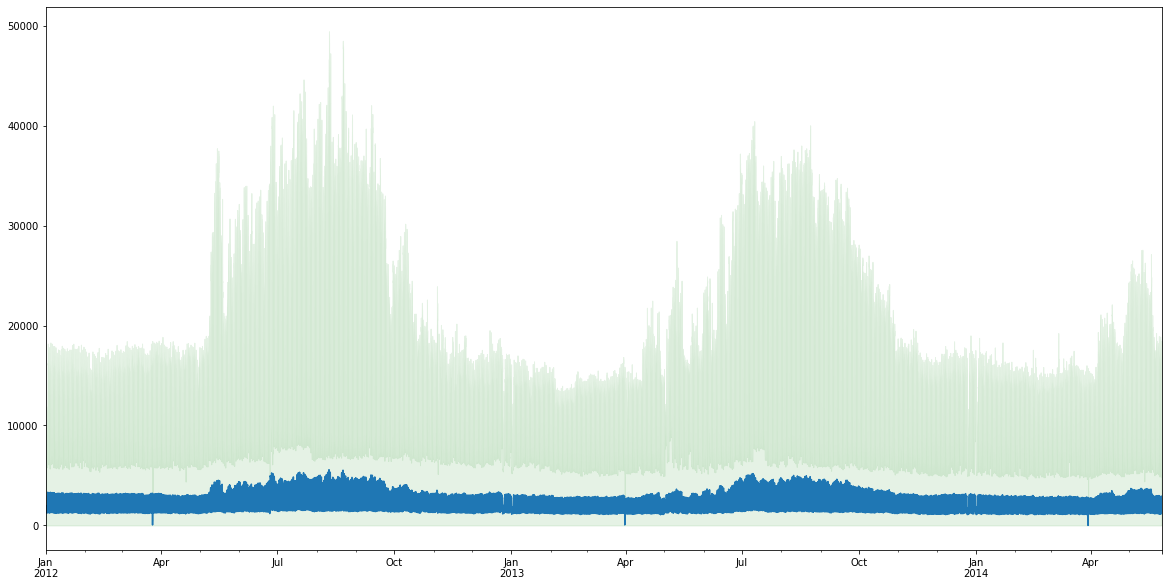
\includegraphics[width=\linewidth]{4_designing/figures/electricity_plot.png}
      \caption{Plot over the average timeseries in the electricity dataset with one standard deviation shown in green. Only positive values are shown as the dataset is non-negative.}
      \label{fig:electricity_plot}
    \endminipage\hfill
\end{figure}

\begin{figure}[htb]
    \centering
    \minipage{1.0\textwidth}
      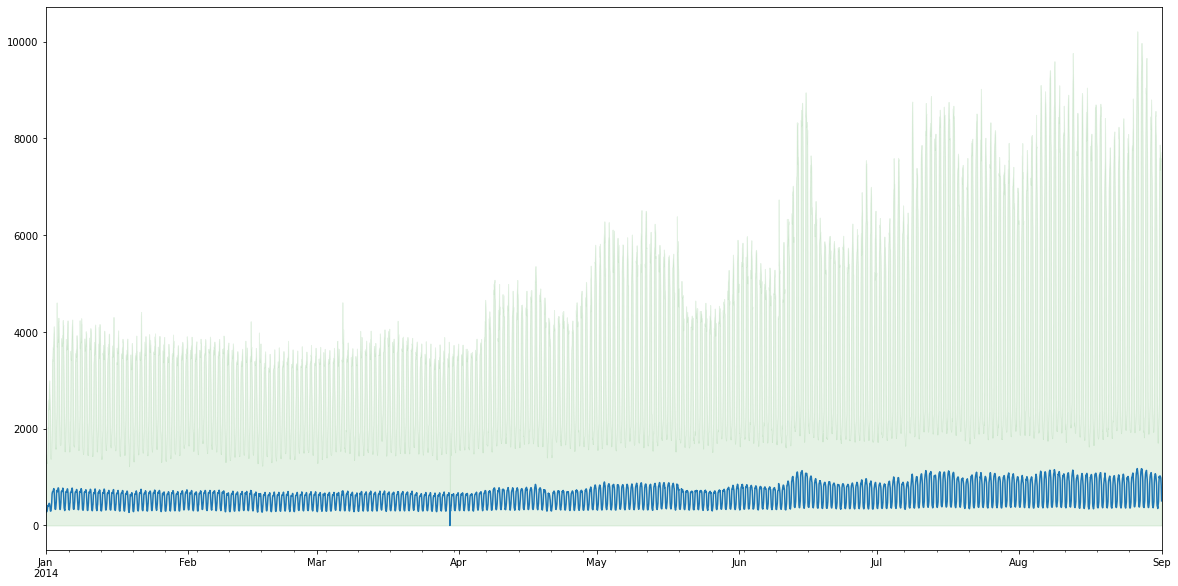
\includegraphics[width=\linewidth]{2_background/figures/electricity_no_negative.png}
      \caption{Zoomed version of \ref{fig:electricity_plot}}
      \label{fig:electricity_plot_zooomed}
    \endminipage\hfill
\end{figure}

\begin{figure}[htb]
    \centering
    \minipage{0.4\textwidth}
        \begin{center}
            \begin{tabular}{||c | c | c | c | c |} 
                \hline
                statistic & mean & deviation & max & min\\
                \hline
                trend & 0.65 & 0.17 & 1.0 & 0.09 \\
                \hline
                seasonality & 0.84 & 0.19 & 1.0 & 0.0 \\
                \hline
                \hline
            \end{tabular}
            \caption{Strength of trend and seasonality of the Electricity dataset}
        \end{center}
    \endminipage\hfill
     \minipage{0.45\textwidth}
      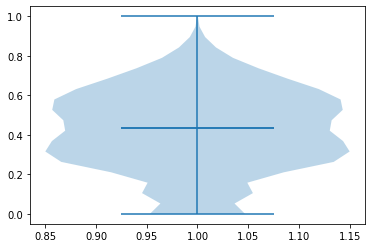
\includegraphics[width=\linewidth]{4_designing/figures/electricity_violin.png}
      \caption{Scaled violin plot of the electricity dataset.}
      \label{fig:electricity_violin}
    \endminipage\hfill
\end{figure}

\clearpage
\subsection{Exchange Rate}

\begin{table}[htb]
    \begin{tabular}{||c | c c c c c c c c ||} 
        \hline
        Dataset & Mean & Series & Items & Shortest & Longest & Min & Max & Frequency\\ [0.5ex] 
        \hline\hline
        train & 0.68 & 8 & 48568 & 6071 & 6071 & 0.01 & 2.11 & 1B\\ 
        \hline
        test & 0.68 & 40 & 246440 & 6101 & 6221 & 0.01 & 2.11 & 1B\\
        \hline
    \end{tabular}
    \caption{Statistics of the Exchange Rate dataset}
\end{table}

\begin{figure}[htb]
    \centering
    \minipage{1.0\textwidth}
      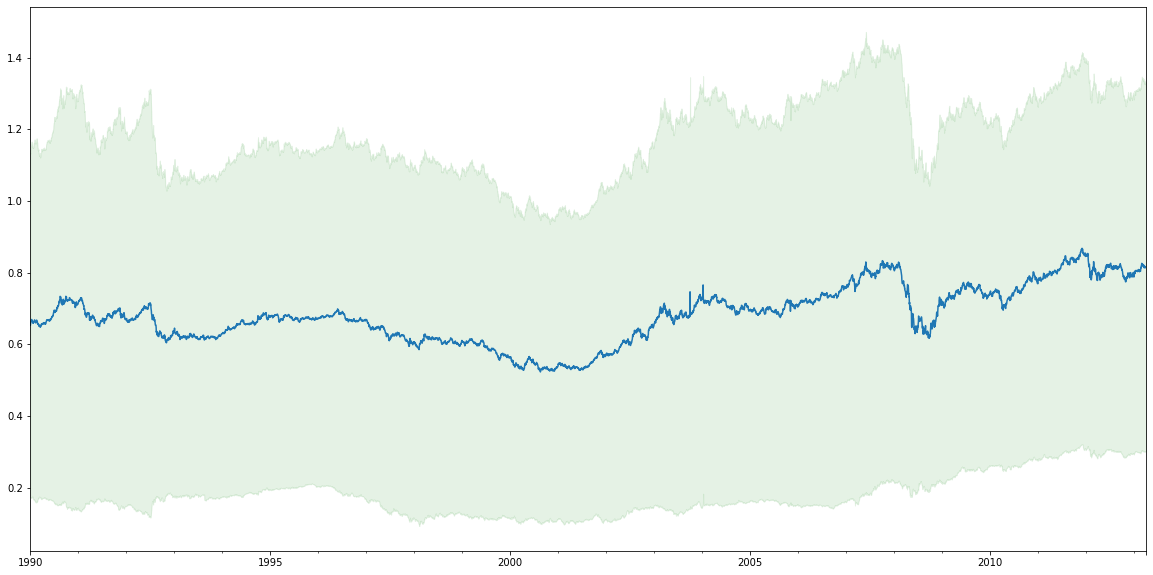
\includegraphics[width=\linewidth]{4_designing/figures/exchange_rate_plot.png}
      \caption{Plot over the average timeseries in the exchange rate dataset with one standard deviation shown in green. Only positive values are shown as the dataset is non-negative.}
      \label{fig:exchange_rate_plot}
    \endminipage\hfill
\end{figure}

\begin{figure}[htb]
    \centering
    \minipage{0.4\textwidth}
        \begin{center}
            \begin{tabular}{||c | c | c | c | c |} 
                \hline
                statistic & mean & deviation & max & min\\
                \hline
                trend & 1.0 & 0.0 & 1.0 & 0.99 \\
                \hline
                seasonality & 0.12 & 0.30 & 0.90 & 0.0 \\
                \hline
                \hline
            \end{tabular}
            \caption{Strength of trend and seasonality of the exchange rate dataset}
        \end{center}
    \endminipage\hfill
     \minipage{0.45\textwidth}
      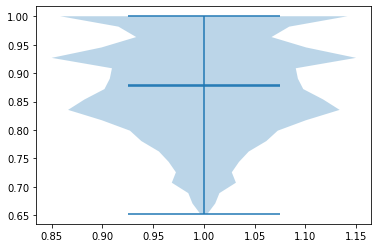
\includegraphics[width=\linewidth]{4_designing/figures/exchange_rate_violin.png}
      \caption{Scaled violin plot of the exchange rate dataset.}
      \label{fig:exchange_rate_violin}
    \endminipage\hfill
\end{figure}

\clearpage
\subsection{Solar Energy}


\begin{table}[htb]
    \begin{tabular}{||c | c c c c c c c c ||} 
        \hline
       Dataset & Mean & Series & Items & Shortest & Longest & Min & Max & Frequency\\ [0.5ex] 
        \hline\hline
        train & 40.35 & 137 & 960233 & 7009 & 7009 & 0.0 & 509.05 & 10min\\ 
        \hline
        test & 40.25 & 959 & 6813695 & 7033 & 7177 & 0.0 & 509.05 & 10min\\
        \hline
    \end{tabular}
    \caption{Statistics of the Solar Energy dataset}
\end{table}


\begin{figure}[htb]
    \centering
    \minipage{1.0\textwidth}
      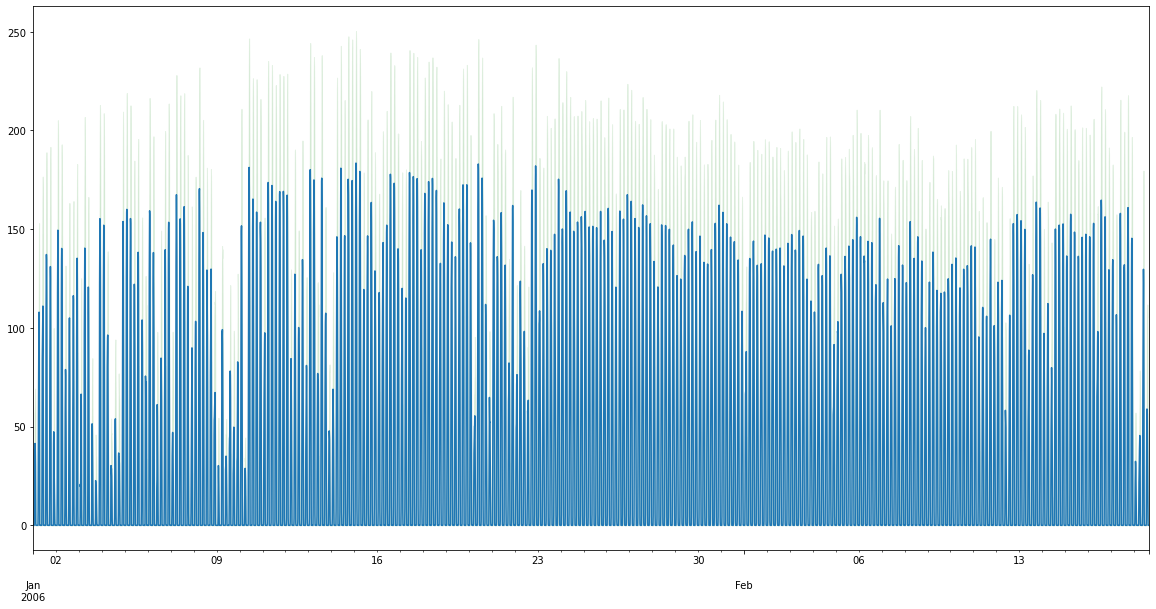
\includegraphics[width=\linewidth]{4_designing/figures/solar-energy_plot.png}
      \caption{Plot over the average timeseries in the solar energy dataset with one standard deviation shown in green. Only positive values are shown as the dataset is non-negative.}
      \label{fig:solar-energy_plot}
    \endminipage\hfill
\end{figure}

\begin{figure}[htb]
    \centering
    \minipage{0.4\textwidth}
        \begin{center}
            \begin{tabular}{||c | c | c | c | c |} 
                \hline
                statistic & mean & deviation & max & min\\
                \hline
                trend & 0.09 & 0.03 & 0.15 & 0.0 \\
                \hline
                seasonality & 0.84 & 0.02 & 0.87 & 0.79 \\
                \hline
                \hline
            \end{tabular}
            \caption{Strength of trend and seasonality of the solar-energy dataset}
        \end{center}
    \endminipage\hfill
     \minipage{0.45\textwidth}
      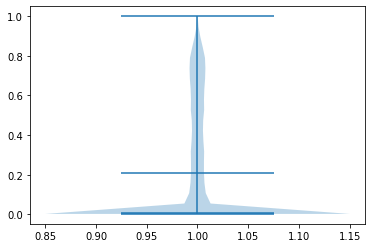
\includegraphics[width=\linewidth]{4_designing/figures/solar-energy_violin.png}
      \caption{Scaled violin plot of the solar energy dataset.}
      \label{fig:solar-energy_violin}
    \endminipage\hfill
\end{figure}

\clearpage
\subsection{Traffic}

\begin{table}[htb]
    \begin{tabular}{||c | c c c c c c c c ||} 
        \hline
       Dataset & Mean & Series & Items & Shortest & Longest & Min & Max & Frequency\\ [0.5ex] 
        \hline\hline
        train & 0.06 & 862 & 12099032 & 14036 & 14036 & 0.0 & 0.72 & H\\ 
        \hline
        test & 0.06 & 6034 & 85272488 & 14060 & 14204 & 0.0 & 0.72 & H\\
        \hline
    \end{tabular}
   \caption{Statistics of the Traffic dataset}
\end{table}

\begin{figure}[htb]
    \centering
    \minipage{1.0\textwidth}
      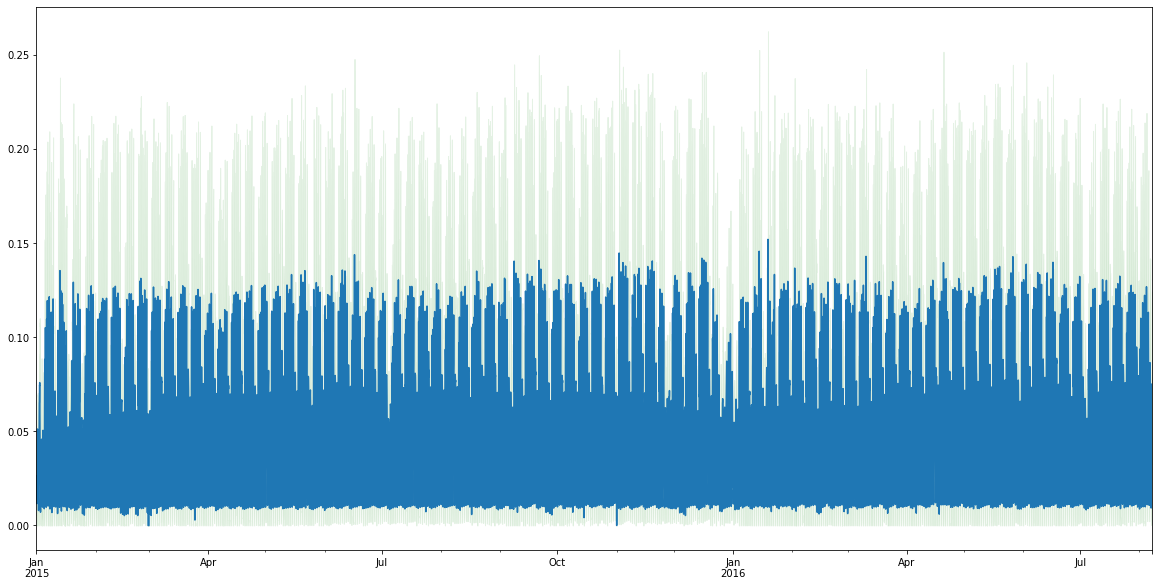
\includegraphics[width=\linewidth]{4_designing/figures/traffic_plot.png}
      \caption{Plot over the average timeseries in the traffic dataset with one standard deviation shown in green. Only positive values are shown as the dataset is non-negative.}
      \label{fig:traffic_plot}
    \endminipage\hfill
\end{figure}

\begin{figure}[htb]
    \centering
    \minipage{0.4\textwidth}
        \begin{center}
            \begin{tabular}{||c | c | c | c | c |} 
                \hline
                statistic & mean & deviation & max & min\\
                \hline
                trend & 0.16 & 0.12 & 0.79 & 0.0 \\
                \hline
                seasonality & 0.67 & 0.10 & 0.93 & 0.12 \\
                \hline
                \hline
            \end{tabular}
            \caption{Strength of trend and seasonality of the traffic dataset}
        \end{center}
    \endminipage\hfill
     \minipage{0.45\textwidth}
      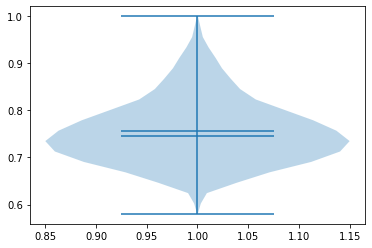
\includegraphics[width=\linewidth]{4_designing/figures/traffic_violin.png}
      \caption{Scaled violin plot of the traffic dataset.}
      \label{fig:traffic_violin}
    \endminipage\hfill
\end{figure}

\clearpage
\subsection{Exchange Rate NIPS}
\begin{table}[htb]
    \begin{tabular}{||c | c c c c c c c c ||} 
        \hline
       Dataset & Mean & Series & Items & Shortest & Longest & Min & Max & Frequency\\ [0.5ex] 
        \hline\hline
        train & 0.68 & 8 & 48568 & 6071 & 6071 & 0.01 & 2.11 & B\\ 
        \hline
        test & 0.68 & 40 & 246440 & 6101 & 6221 & 0.01 & 2.11 & B\\
        \hline
    \end{tabular}
   \caption{Statistics of the Exchange Rate NIPS dataset}    
\end{table}

\begin{figure}[htb]
    \centering
    \minipage{1.0\textwidth}
      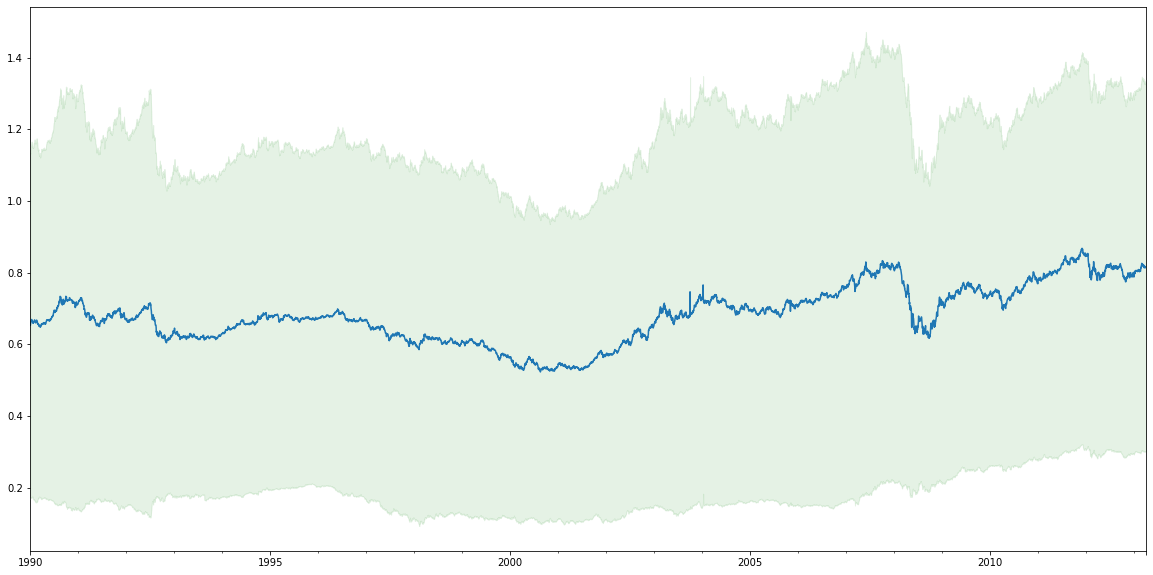
\includegraphics[width=\linewidth]{4_designing/figures/exchange_rate_nips_plot.png}
      \caption{Plot over the average timeseries in the exchange rate nips dataset with one standard deviation shown in green. Only positive values are shown as the dataset is non-negative.}
      \label{fig:exchange_rate_nips_plot}
    \endminipage\hfill
\end{figure}

\begin{figure}[htb]
    \centering
    \minipage{0.4\textwidth}
        \begin{center}
            \begin{tabular}{||c | c | c | c | c |} 
                \hline
                statistic & mean & deviation & max & min\\
                \hline
                trend & 1.0 & 0.0 & 1.0 & 0.99 \\
                \hline
                seasonality & 0.12 & 0.30 & 0.90 & 0.0 \\
                \hline
                \hline
            \end{tabular}
            \caption{Strength of trend and seasonality of the exchange rate nips dataset}
        \end{center}
    \endminipage\hfill
     \minipage{0.45\textwidth}
      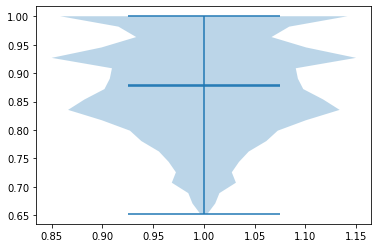
\includegraphics[width=\linewidth]{4_designing/figures/exchange_rate_nips_violin.png}
      \caption{Scaled violin plot of the exchange rate nips dataset.}
      \label{fig:exchange_rate_nips_violin}
    \endminipage\hfill
\end{figure}

\clearpage
\subsection{Electricity NIPS}
 \begin{table}[htb]
    \begin{tabular}{||c | c c c c c c c c ||} 
        \hline
       Dataset & Mean & Series & Items & Shortest & Longest & Min & Max & Frequency\\ [0.5ex] 
        \hline\hline
        train & 607.95 & 370 & 2142282 & 1081 & 5833 & 0.0 & 168100.0 & H\\ 
        \hline
        test & 652.36 & 2590 & 10340239 & 1105 & 4000 & 0.0 & 168100.0 & H\\
        \hline
    \end{tabular}
    \caption{Statistics of the Electricity NIPS dataset.}
\end{table}

\begin{figure}[htb]
    \centering
    \minipage{1.0\textwidth}
      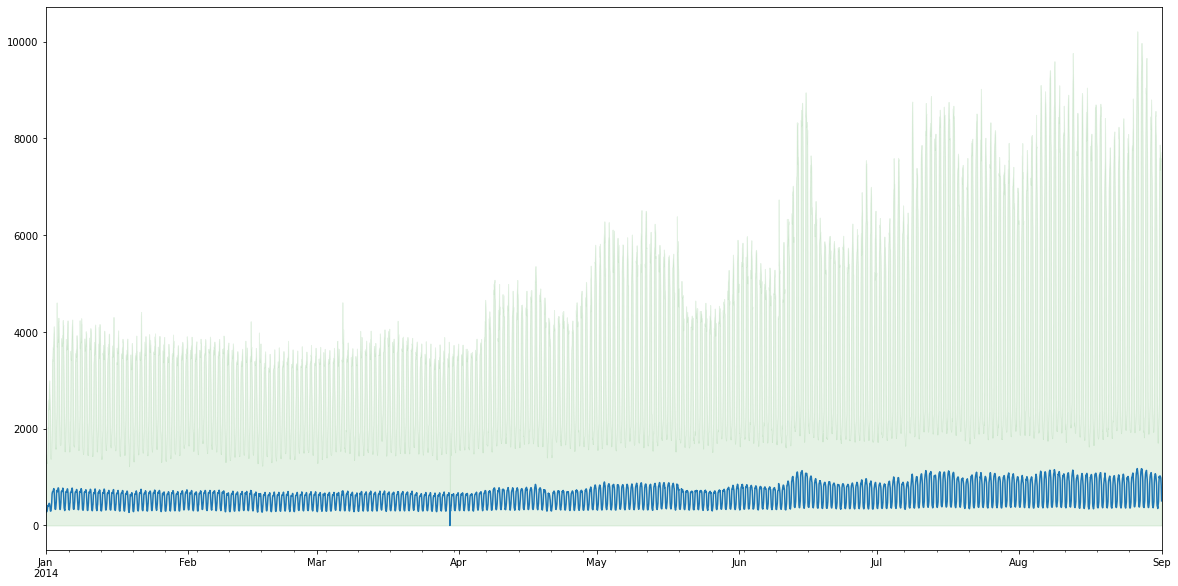
\includegraphics[width=\linewidth]{4_designing/figures/electricity_nips_plot.png}
      \caption{Plot over the average timeseries in the electricity nips dataset with one standard deviation shown in green. Only positive values are shown as the dataset is non-negative.}
      \label{fig:electricity_nips_plot}
    \endminipage\hfill
\end{figure}

\begin{figure}[htb]
    \centering
    \minipage{0.4\textwidth}
        \begin{center}
            \begin{tabular}{||c | c | c | c | c |} 
                \hline
                statistic & mean & deviation & max & min\\
                \hline
                trend & 0.54 & 0.20 & 1.0 & 0.0 \\
                \hline
                seasonality & 0.86 & 0.16 & 1.0 & 0.0 \\
                \hline
                \hline
            \end{tabular}
            \caption{Strength of trend and seasonality of the electricity nips dataset}
        \end{center}
    \endminipage\hfill
     \minipage{0.45\textwidth}
      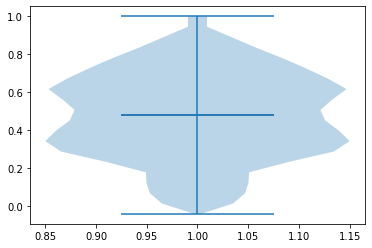
\includegraphics[width=\linewidth]{4_designing/figures/electricity_nips_violin.png}
      \caption{Scaled violin plot of the electricity nips dataset.}
      \label{fig:electricity_nips_violin}
    \endminipage\hfill
\end{figure}

\clearpage
\subsection{Solar Energy NIPS}
\begin{table}[htb]
    \begin{tabular}{||c | c c c c c c c c ||} 
        \hline
       Dataset & Mean & Series & Items & Shortest & Longest & Min & Max & Frequency\\ [0.5ex] 
        \hline\hline
        train & 40.35 & 137 & 960233 & 7009 & 7009 & 0.00 & 509.05 & H\\ 
        \hline
        test & 40.25 & 959 & 6813695 & 7033 & 7177 & 0.00 & 509.05 & H\\
        \hline
    \end{tabular}
   \caption{Statistics of the Solar Energy NIPS dataset}
\end{table}

\begin{figure}[htb]
    \centering
    \minipage{1.0\textwidth}
      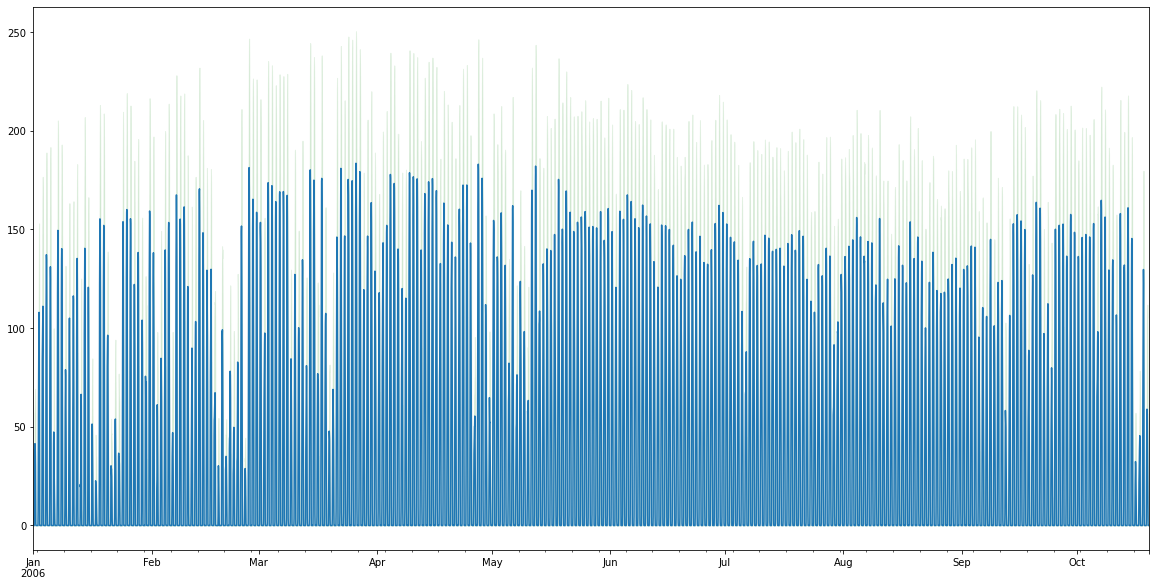
\includegraphics[width=\linewidth]{4_designing/figures/solar_nips_plot.png}
      \caption{Plot over the average timeseries in the solar nips dataset with one standard deviation shown in green. Only positive values are shown as the dataset is non-negative.}
      \label{fig:solar_nips_plot}
    \endminipage\hfill
\end{figure}

\begin{figure}[htb]
    \centering
    \minipage{0.4\textwidth}
        \begin{center}
            \begin{tabular}{||c | c | c | c | c |} 
                \hline
                statistic & mean & deviation & max & min\\
                \hline
                trend & 0.17 & 0.02 & 0.24 & 0.11 \\
                \hline
                seasonality & 0.86 & 0.02 & 0.89 & 0.80 \\
                \hline
                \hline
            \end{tabular}
            \caption{Strength of trend and seasonality of the solar nips dataset}
        \end{center}
    \endminipage\hfill
     \minipage{0.45\textwidth}
      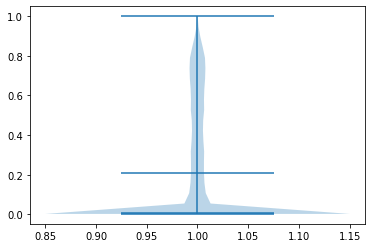
\includegraphics[width=\linewidth]{4_designing/figures/solar_nips_violin.png}
      \caption{Scaled violin plot of the solar nips dataset.}
      \label{fig:solar_nips_violin}
    \endminipage\hfill
\end{figure}


\clearpage
\subsection{Traffic NIPS}
\begin{table}[htb]
    \begin{tabular}{||c | c c c c c c c c ||} 
        \hline
       Dataset & Mean & Series & Items & Shortest & Longest & Min & Max & Frequency\\ [0.5ex] 
        \hline\hline
        train & 0.05 & 963 & 3852963 & 4001 & 4001 & 0.00 & 1.00 & H\\ 
        \hline
        test & 0.05 & 6741 & 26964000 & 4000 & 4000 & 0.00 & 1.00 & H\\
        \hline
    \end{tabular}
   \caption{Statistics of the Traffic NIPS dataset}
\end{table}


\begin{figure}[htb]
    \centering
    \minipage{1.0\textwidth}
      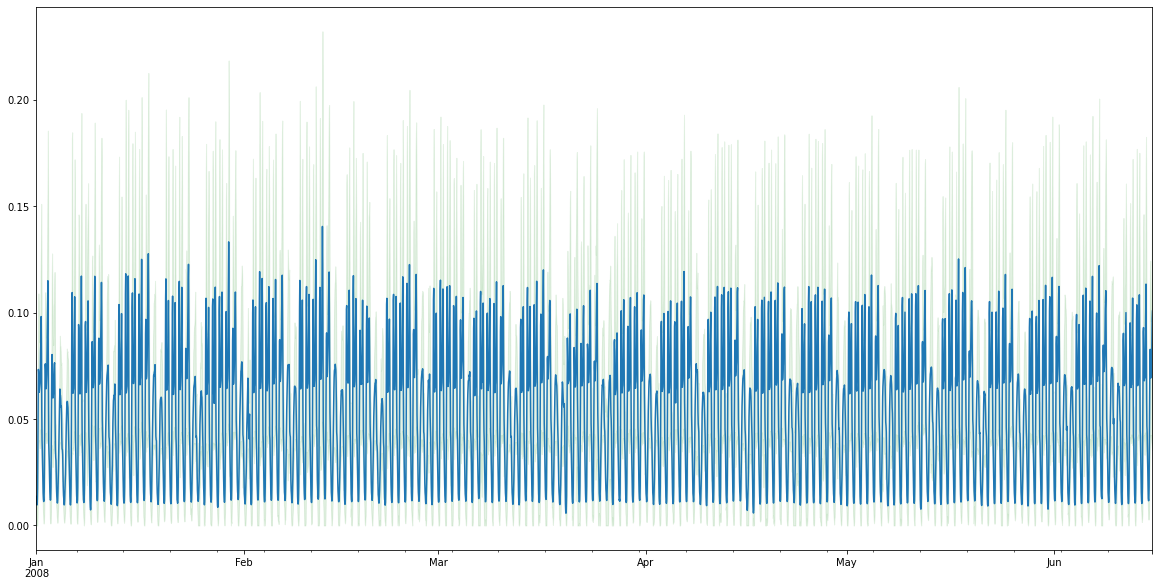
\includegraphics[width=\linewidth]{4_designing/figures/traffic_nips_plot.png}
      \caption{Plot over the average timeseries in the traffic nips dataset with one standard deviation shown in green. Only positive values are shown as the dataset is non-negative.}
      \label{fig:traffic_nips_plot}
    \endminipage\hfill
\end{figure}

\begin{figure}[htb]
    \centering
    \minipage{0.4\textwidth}
        \begin{center}
            \begin{tabular}{||c | c | c | c | c |} 
                \hline
                statistic & mean & deviation & max & min\\
                \hline
                trend & 0.29 & 0.18 & 0.87 & 0.0 \\
                \hline
                seasonality & 0.76 & 0.12 & 0.94 & 0.0 \\
                \hline
                \hline
            \end{tabular}
            \caption{Strength of trend and seasonality of the traffic nips dataset}
        \end{center}
    \endminipage\hfill
     \minipage{0.45\textwidth}
      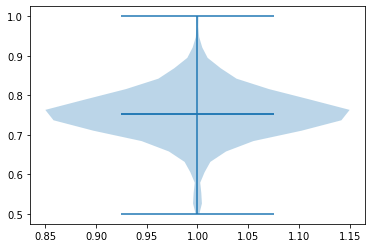
\includegraphics[width=\linewidth]{4_designing/figures/traffic_nips_violin.png}
      \caption{Scaled violin plot of the traffic nips dataset.}
      \label{fig:traffic_nips_violin}
    \endminipage\hfill
\end{figure}
\clearpage
\subsection{Wiki Rolling NIPS}

\begin{table}[htb]
    \begin{tabular}{||c | c c c c c c c c ||} 
        \hline
       Dataset & Mean & Series & Items & Shortest & Longest & Min & Max & Frequency\\ [0.5ex] 
        \hline\hline
        train & 3720.54 & 9535 & 7551720 & 792 & 792 & 0.00 & 7752515.00 & D\\ 
        \hline
        test & 3663.55 & 47675 & 40619100 & 792 & 912 & 0.00 & 7752515.00 & D\\
        \hline
    \end{tabular}
   \caption{Statistics of the Wiki Rolling NIPS dataset}
\end{table}


\begin{figure}[htb]
    \centering
    \minipage{1.0\textwidth}
      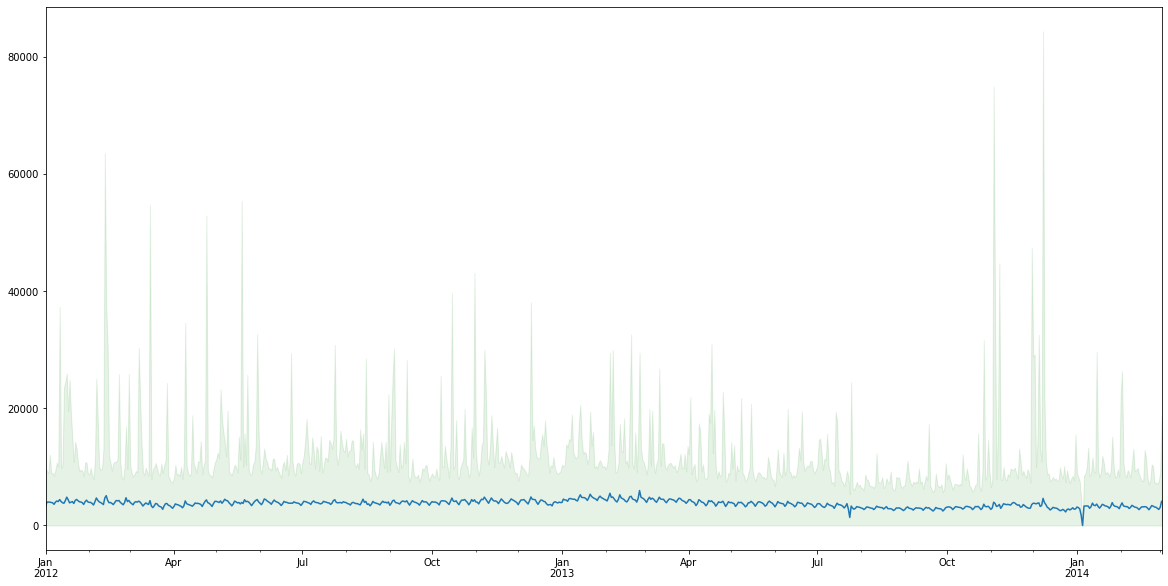
\includegraphics[width=\linewidth]{4_designing/figures/wiki-rolling_nips_plot.png}
      \caption{Plot over the average timeseries in the wiki-rolling nips dataset with one standard deviation shown in green. Only positive values are shown as the dataset is non-negative.}
      \label{fig:wiki-rolling_nips_plot}
    \endminipage\hfill
\end{figure}

\begin{figure}[htb]
    \centering
    \minipage{0.4\textwidth}
        \begin{center}
            \begin{tabular}{||c | c | c | c | c |} 
                \hline
                statistic & mean & deviation & max & min\\
                \hline
                trend & 0.53 & 0.27 & 1.0 & 0.0 \\
                \hline
                seasonality & 0.23 & 0.26 & 1.0 & 0.0 \\
                \hline
                \hline
            \end{tabular}
            \caption{Strength of trend and seasonality of the wiki-rolling nips dataset}
        \end{center}
    \endminipage\hfill
     \minipage{0.45\textwidth}
      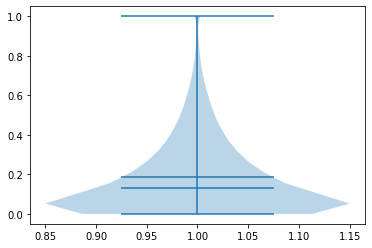
\includegraphics[width=\linewidth]{4_designing/figures/wiki-rolling_nips_violin.png}
      \caption{Scaled violin plot of the wiki-rolling nips dataset.}
      \label{fig:wiki-rolling_nips_violin}
    \endminipage\hfill
\end{figure}

\clearpage
\subsection{Taxi}
\begin{table}[htb]
    \begin{tabular}{||c | c c c c c c c c ||} 
        \hline
       Dataset & Mean & Series & Items & Shortest & Longest & Min & Max & Frequency\\ [0.5ex] 
        \hline\hline
        train & 8.79 & 1214 & 1806432 & 1488 & 1488 & 0.0 & 265.0 & 30min\\ 
        \hline
        test & 7.41 & 67984 & 54999056 & 149 & 1469 & 0.0 & 225.0 & 30min\\
        \hline
    \end{tabular}
    \caption{Statistics of the Taxi NIPS dataset}
\end{table}

\begin{figure}[htb]
    \centering
    \minipage{1.0\textwidth}
      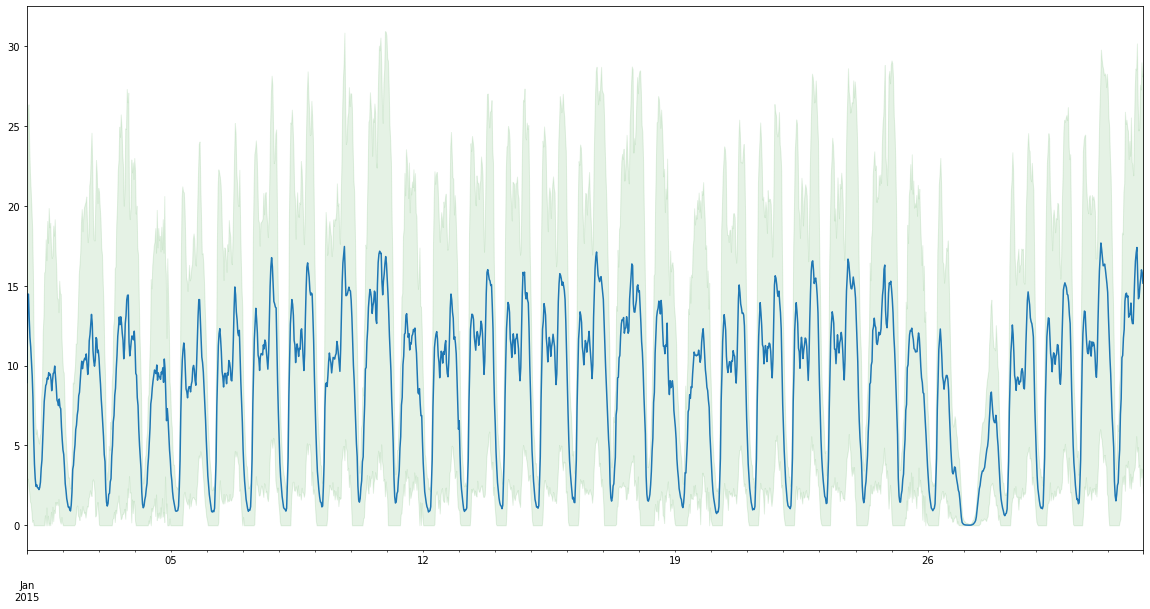
\includegraphics[width=\linewidth]{4_designing/figures/taxi_30min_plot.png}
      \caption{Plot over the average timeseries in the taxi dataset with one standard deviation shown in green. Only positive values are shown as the dataset is non-negative.}
      \label{fig:taxi_30min_plot}
    \endminipage\hfill
\end{figure}

\begin{figure}[htb]
    \centering
    \minipage{0.4\textwidth}
        \begin{center}
            \begin{tabular}{||c | c | c | c | c |} 
                \hline
                statistic & mean & deviation & max & min\\
                \hline
                trend & 0.02 & 0.02 & 0.16 & 0.0 \\
                \hline
                seasonality & 0.66 & 0.08 & 0.92 & 0.41 \\
                \hline
                \hline
            \end{tabular}
            \caption{Strength of trend and seasonality of the taxi dataset}
        \end{center}
    \endminipage\hfill
     \minipage{0.45\textwidth}
      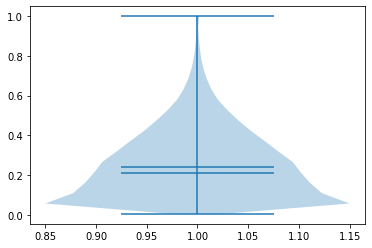
\includegraphics[width=\linewidth]{4_designing/figures/taxi_30min_violin.png}
      \caption{Scaled violin plot of the taxi dataset.}
      \label{fig:taxi_30min_violin}
    \endminipage\hfill
\end{figure}

\clearpage
\subsection{M3 Monthly}

\begin{table}[htb]
    \begin{tabular}{||c | c c c c c c c ||} 
        \hline
        Dataset & Mean & Series & Items & Shortest & Longest & Min & Max \\ [0.5ex] 
        \hline\hline
        train & 4928.47 & 1428 & 141858 & 48 & 126 & 80.00 & 86730.00\\ 
        \hline
        test & 4971.28 & 1428 & 167562 & 66 & 144 & -1200.00 & 86730.00\\
        \hline
    \end{tabular}
    \caption{Statistics of the M3 Monthly dataset.}
\end{table}

\begin{figure}[htb]
    \centering
    \minipage{1.0\textwidth}
      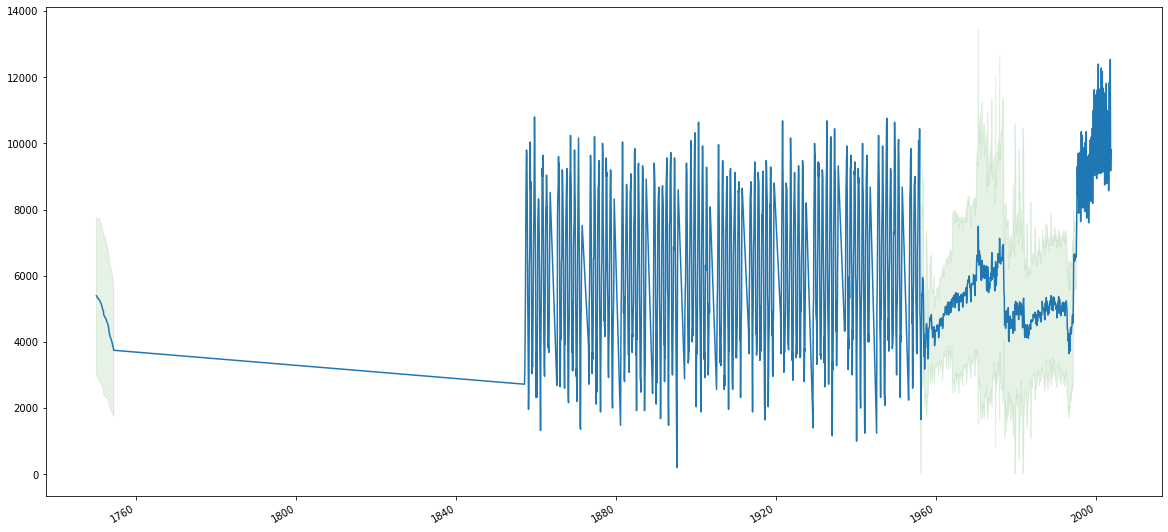
\includegraphics[width=\linewidth]{4_designing/figures/m3_monthly_plot.png}
      \caption{Plot over the average timeseries in the m3 monthly dataset with one standard deviation shown in green. Only positive values are shown as the dataset is non-negative.}
      \label{fig:m3_monthly_plot}
    \endminipage\hfill
\end{figure}

\begin{figure}[htb]
    \centering
    \minipage{0.4\textwidth}
        \begin{center}
            \begin{tabular}{||c | c | c | c | c |} 
                \hline
                statistic & mean & deviation & max & min\\
                \hline
                trend & 0.68 & 0.31 & 1.0 & 0.0 \\
                \hline
                seasonality & 0.35 & 0.29 & 1.0 & 0.0 \\
                \hline
                \hline
            \end{tabular}
            \caption{Strength of trend and seasonality of the m3 monthly dataset}
        \end{center}
    \endminipage\hfill
     \minipage{0.45\textwidth}
      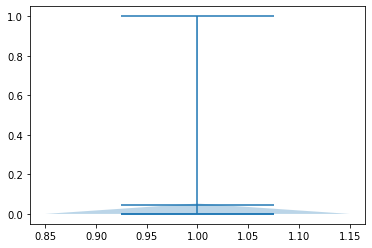
\includegraphics[width=\linewidth]{4_designing/figures/m3_monthly_violin.png}
      \caption{Scaled violin plot of the m3 monthly dataset.}
      \label{fig:m3_monthly_violin}
    \endminipage\hfill
\end{figure}

\clearpage
\subsection{M3 Quarterly}
\begin{table}[htb]
    \begin{tabular}{||c | c c c c c c c ||} 
        \hline
        Dataset & Mean & Series & Items & Shortest & Longest & Min & Max \\ [0.5ex] 
        \hline\hline
        train & 4819.27 & 756 & 30956 & 16 & 64 & 126.00 & 20245.00\\ 
        \hline
        test & 4983.53 & 756 & 37004 & 24 & 72 & 121.00 & 20375.00\\
        \hline
    \end{tabular}
    \caption{Statistics of the M3 Quarterly dataset.}
\end{table}
\begin{figure}[htb]
    \centering
    \minipage{1.0\textwidth}
      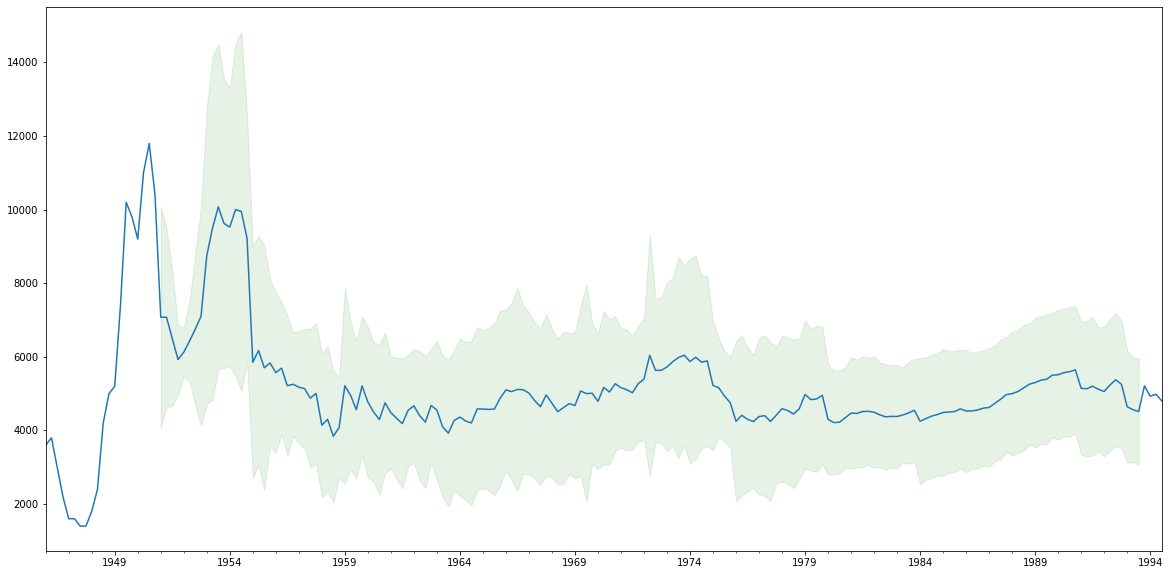
\includegraphics[width=\linewidth]{4_designing/figures/m3_quarterly_plot.png}
      \caption{Plot over the average timeseries in the m3 quarterly dataset with one standard deviation shown in green. Only positive values are shown as the dataset is non-negative.}
      \label{fig:m3_quarterly_plot}
    \endminipage\hfill
\end{figure}

\begin{figure}[htb]
    \centering
    \minipage{0.4\textwidth}
        \begin{center}
            \begin{tabular}{||c | c | c | c | c |} 
                \hline
                statistic & mean & deviation & max & min\\
                \hline
                trend & 0.88 & 0.19 & 1.0 & 0.0 \\
                \hline
                seasonality & 0.33 & 0.35 & 1.0 & 0.0 \\
                \hline
                \hline
            \end{tabular}
            \caption{Strength of trend and seasonality of the m3 quarterly dataset}
        \end{center}
    \endminipage\hfill
     \minipage{0.45\textwidth}
      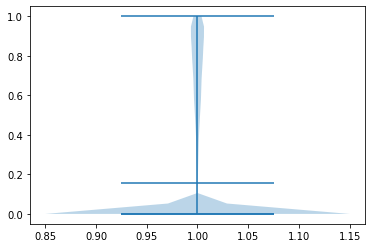
\includegraphics[width=\linewidth]{4_designing/figures/m3_quarterly_violin.png}
      \caption{Scaled violin plot of the m3 quarterly dataset.}
      \label{fig:m3_quarterly_violin}
    \endminipage\hfill
\end{figure}

\clearpage
\subsection{M3 Yearly}
\begin{table}[htb]
    \begin{tabular}{||c | c c c c c c c ||} 
        \hline
        Dataset & Mean & Series & Items & Shortest & Longest & Min & Max \\ [0.5ex] 
        \hline\hline
        train & 4417.05 & 645 & 14449 & 14 & 41 & 30.00 & 39666.22\\ 
        \hline
        test & 4815.77 & 645 & 18319 & 20 & 47 & 30.00 & 45525.66\\
        \hline
    \end{tabular}
\caption{Statistics of the M3 Yearly dataset}
\end{table}
\begin{figure}[htb]
    \centering
    \minipage{1.0\textwidth}
      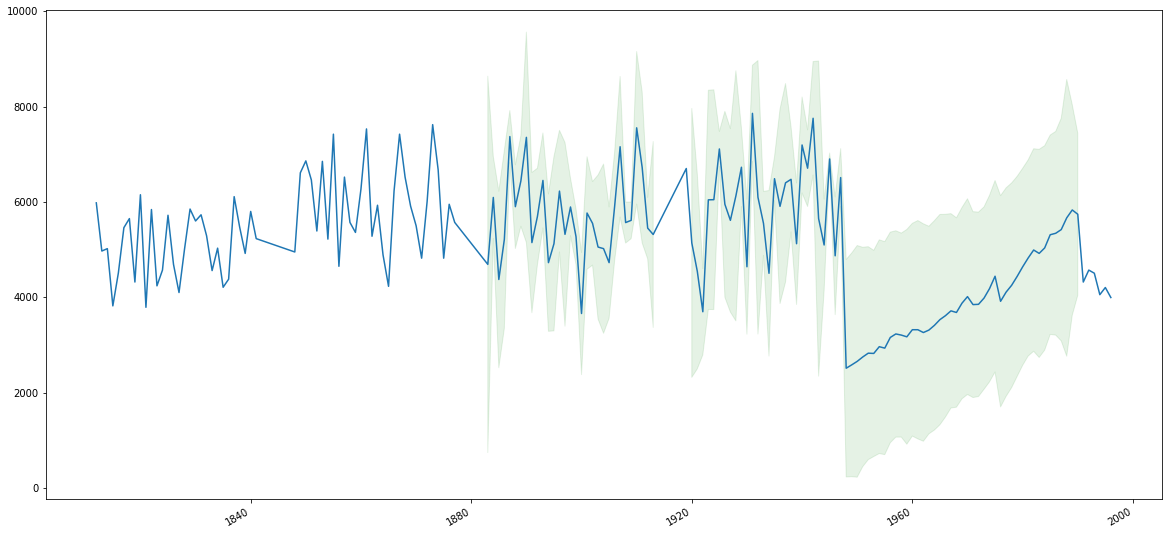
\includegraphics[width=\linewidth]{4_designing/figures/m3_yearly_plot.png}
      \caption{Plot over the average timeseries in the m3 yearly dataset with one standard deviation shown in green. Only positive values are shown as the dataset is non-negative.}
      \label{fig:m3_yearly_plot}
    \endminipage\hfill
\end{figure}

\begin{figure}[htb]
    \centering
    \minipage{0.4\textwidth}
        \begin{center}
            \begin{tabular}{||c | c | c | c | c |} 
                \hline
                statistic & mean & deviation & max & min\\
                \hline
                trend & 0.89 & 0.17 & 1.0 & 0.0 \\
                \hline
                seasonality & 0.09 & 0.17 & 0.96 & 0.0 \\
                \hline
                \hline
            \end{tabular}
            \caption{Strength of trend and seasonality of the m3 yearly dataset}
        \end{center}
    \endminipage\hfill
     \minipage{0.45\textwidth}
      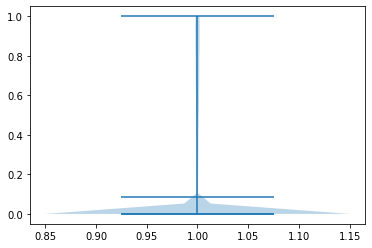
\includegraphics[width=\linewidth]{4_designing/figures/m3_yearly_violin.png}
      \caption{Scaled violin plot of the m3 yearly dataset.}
      \label{fig:m3_yearly_violin}
    \endminipage\hfill
\end{figure}

\clearpage
\subsection{M3 Other}
\begin{table}[htb]
    \begin{tabular}{||c | c c c c c c c ||} 
        \hline
        Dataset & Mean & Series & Items & Shortest & Longest & Min & Max \\ [0.5ex] 
        \hline\hline
        train & 6152.18 & 174 & 11933 & 63 & 96 & 28.00 & 59472.00\\ 
        \hline
        test & 5999.87 & 174 & 13325 & 71 & 104 & 28.00 & 59472.00\\
        \hline
    \end{tabular}
\caption{Statistics of the M3 Other dataset}
\end{table}
    
\begin{figure}[htb]
    \centering
    \minipage{1.0\textwidth}
      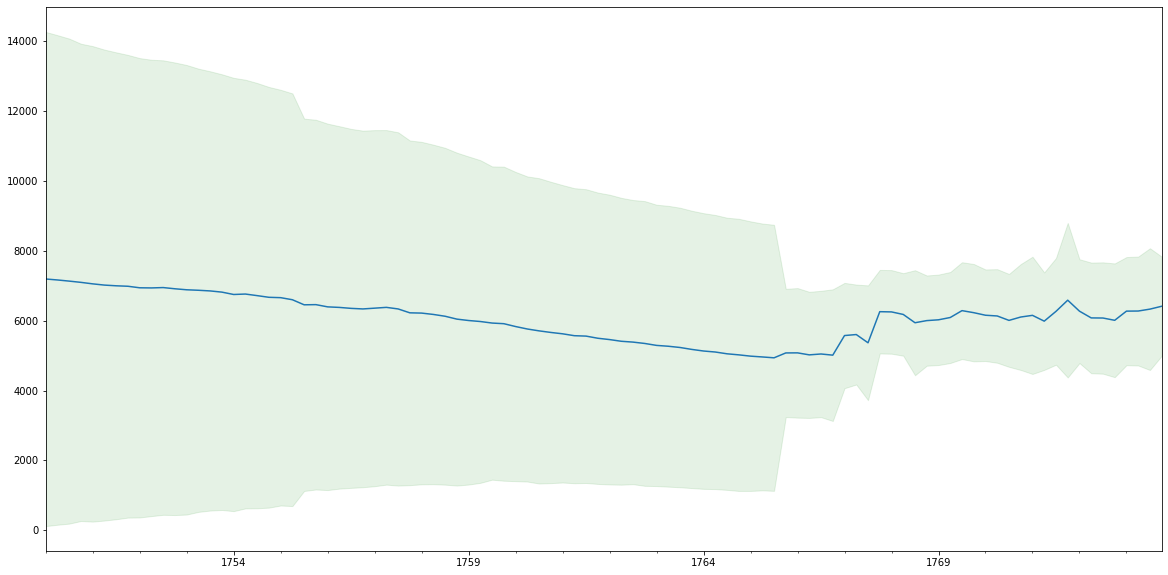
\includegraphics[width=\linewidth]{4_designing/figures/m3_other_plot.png}
      \caption{Plot over the average timeseries in the m3 other dataset with one standard deviation shown in green. Only positive values are shown as the dataset is non-negative.}
      \label{fig:m3_other_plot}
    \endminipage\hfill
\end{figure}

\begin{figure}[htb]
    \centering
    \minipage{0.4\textwidth}
        \begin{center}
            \begin{tabular}{||c | c | c | c | c |} 
                \hline
                statistic & mean & deviation & max & min\\
                \hline
                trend & 0.94 & 0.17 & 1.0 & 0.35 \\
                \hline
                seasonality & 0.07 & 0.08 & 0.44 & 0.0 \\
                \hline
                \hline
            \end{tabular}
            \caption{Strength of trend and seasonality of the m3 other dataset}
        \end{center}
    \endminipage\hfill
     \minipage{0.45\textwidth}
      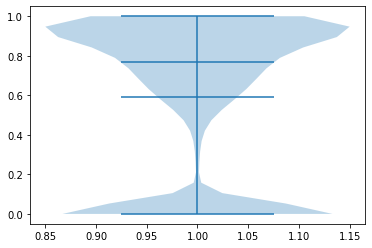
\includegraphics[width=\linewidth]{4_designing/figures/m3_other_violin.png}
      \caption{Scaled violin plot of the m3 other dataset.}
      \label{fig:m3_other_violin}
    \endminipage\hfill
\end{figure}

\clearpage
\subsection{M4 Hourly}

\begin{table}[htb]
    \begin{tabular}{||c | c c c c c c c c ||} 
        \hline
       Dataset & Mean & Series & Items & Shortest & Longest & Min & Max & Frequency\\ [0.5ex] 
        \hline\hline
        train & 6827.69 & 414 & 353500 & 700 & 960 & 10.00 & 703008.00 & H\\ 
        \hline
        test & 6859.56 & 414 & 373372 & 748 & 1008 & 10.00 & 703008.00 & H\\
        \hline
    \end{tabular}
    \caption{Statistics of the M4 Hourly dataset}
\end{table}


\begin{figure}[htb]
    \centering
    \minipage{1.0\textwidth}
      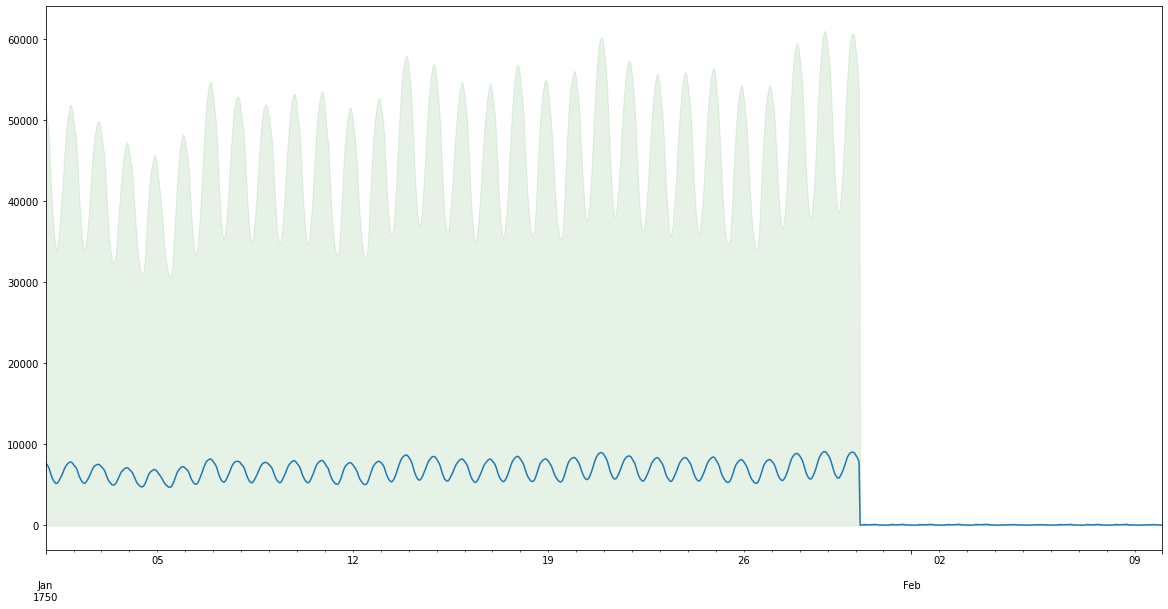
\includegraphics[width=\linewidth]{4_designing/figures/m4_hourly_plot.png}
      \caption{Plot over the average timeseries in the m4 hourly dataset with one standard deviation shown in green. Only positive values are shown as the dataset is non-negative.}
      \label{fig:m4_hourly_plot}
    \endminipage\hfill
\end{figure}

\begin{figure}[htb]
    \centering
    \minipage{0.4\textwidth}
        \begin{center}
            \begin{tabular}{||c | c | c | c | c |} 
                \hline
                statistic & mean & deviation & max & min\\
                \hline
                trend & 0.62 & 0.37 & 1.0 & 0.0 \\
                \hline
                seasonality & 0.88 & 0.16 & 1.0 & 0.0 \\
                \hline
                \hline
            \end{tabular}
            \caption{Strength of trend and seasonality of the m4 hourly dataset}
        \end{center}
    \endminipage\hfill
     \minipage{0.45\textwidth}
      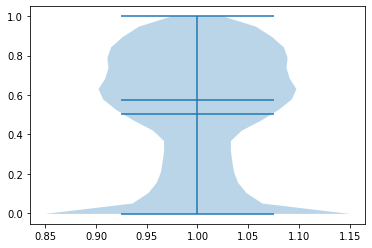
\includegraphics[width=\linewidth]{4_designing/figures/m4_hourly_violin.png}
      \caption{Scaled violin plot of the m4 hourly dataset.}
      \label{fig:m4_hourly_violin}
    \endminipage\hfill
\end{figure}


\clearpage
\subsection{M4 Daily}
\begin{table}[htb]
    \begin{tabular}{||c | c c c c c c c c ||} 
        \hline
       Dataset & Mean & Series & Items & Shortest & Longest & Min & Max & Frequency\\ [0.5ex] 
        \hline\hline
        train & 4951.40 & 4227 & 9964658 & 93 & 9919 & 15.00 & 352000.00 & D\\ 
        \hline
        test & 4960.15 & 4227 & 10023836 & 107 & 9933 & 15.00 & 352000.00 & D\\
        \hline
    \end{tabular}
    \caption{Statistics of the M4 Daily dataset}
\end{table}

\begin{figure}[htb]
    \centering
    \minipage{1.0\textwidth}
      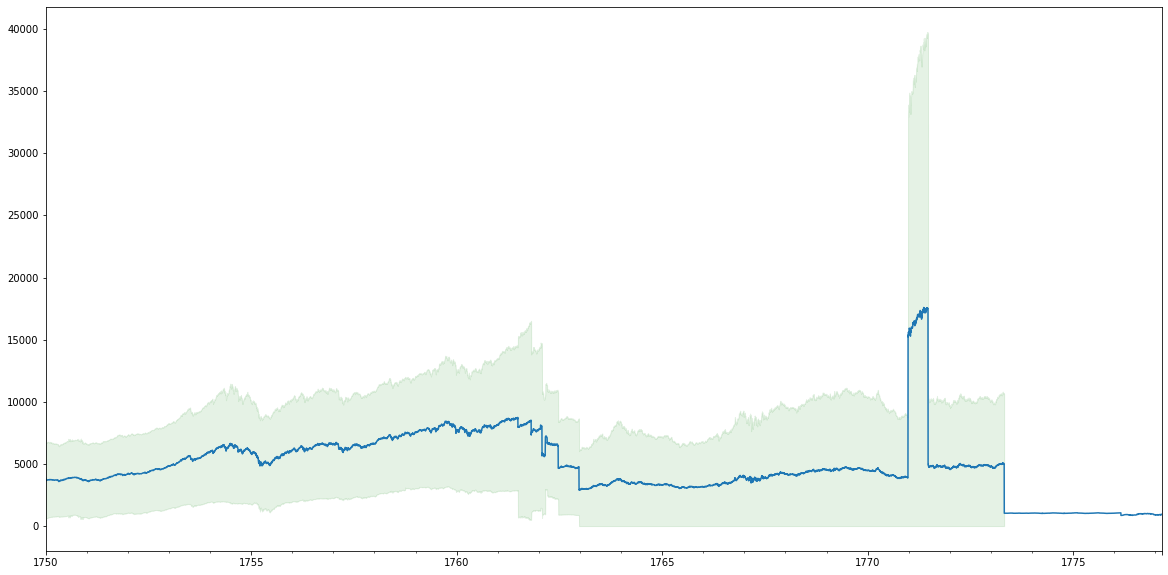
\includegraphics[width=\linewidth]{4_designing/figures/m4_daily_plot.png}
      \caption{Plot over the average timeseries in the m4 daily dataset with one standard deviation shown in green. Only positive values are shown as the dataset is non-negative.}
      \label{fig:m4_daily_plot}
    \endminipage\hfill
\end{figure}

\begin{figure}[htb]
    \centering
    \minipage{0.4\textwidth}
        \begin{center}
            \begin{tabular}{||c | c | c | c | c |} 
                \hline
                statistic & mean & deviation & max & min\\
                \hline
                trend & 0.98 & 0.05 & 1.0 & 0.0 \\
                \hline
                seasonality & 0.05 & 0.10 & 1.0 & 0.0 \\
                \hline
                \hline
            \end{tabular}
            \caption{Strength of trend and seasonality of the m4 daily dataset}
        \end{center}
    \endminipage\hfill
     \minipage{0.45\textwidth}
      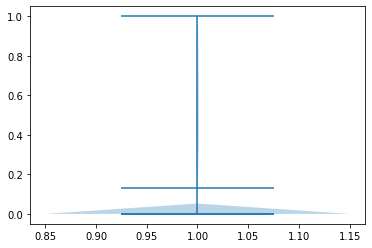
\includegraphics[width=\linewidth]{4_designing/figures/m4_daily_violin.png}
      \caption{Scaled violin plot of the m4 daily dataset.}
      \label{fig:m4_daily_violin}
    \endminipage\hfill
\end{figure}

\clearpage
\subsection{M4 Weekly}
\begin{table}[htb]
    \begin{tabular}{||c | c c c c c c c c ||} 
        \hline
       Dataset & Mean & Series & Items & Shortest & Longest & Min & Max & Frequency\\ [0.5ex] 
        \hline\hline
        train & 3738.52 & 359 & 366912 & 80 & 2597 & 104.69 & 51410.00 & W\\ 
        \hline
        test & 3755.97 & 359 & 371579 & 93 & 2610 & 104.69 & 51410.00 & W\\
        \hline
    \end{tabular}
    \caption{Statistics of the M4 Weekly dataset}
\end{table}

\begin{figure}[htb]
    \centering
    \minipage{1.0\textwidth}
      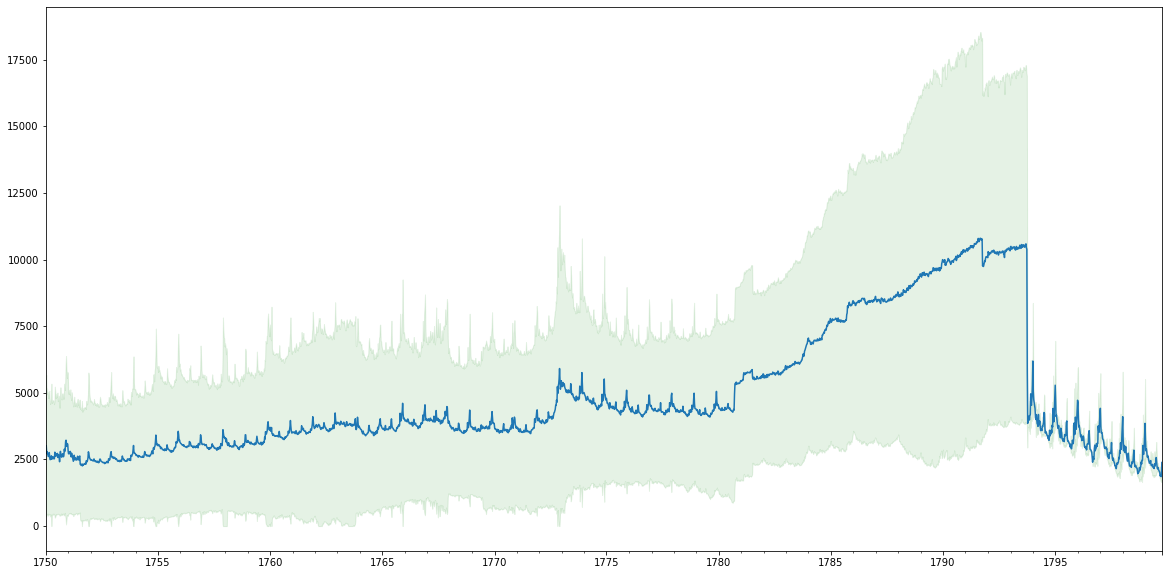
\includegraphics[width=\linewidth]{4_designing/figures/m4_weekly_plot.png}
      \caption{Plot over the average timeseries in the m4 weekly dataset with one standard deviation shown in green. Only positive values are shown as the dataset is non-negative.}
      \label{fig:m4_weekly_plot}
    \endminipage\hfill
\end{figure}

\begin{figure}[htb]
    \centering
    \minipage{0.4\textwidth}
        \begin{center}
            \begin{tabular}{||c | c | c | c | c |} 
                \hline
                statistic & mean & deviation & max & min\\
                \hline
                trend & 0.77 & 0.31 & 1.0 & 0.0 \\
                \hline
                seasonality & 0.34 & 0.35 & 1.0 & 0.0 \\
                \hline
                \hline
            \end{tabular}
            \caption{Strength of trend and seasonality of the m4 weekly dataset}
        \end{center}
    \endminipage\hfill
     \minipage{0.45\textwidth}
      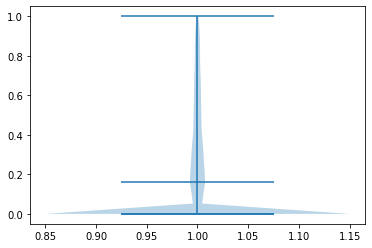
\includegraphics[width=\linewidth]{4_designing/figures/m4_weekly_violin.png}
      \caption{Scaled violin plot of the m4 weekly dataset.}
      \label{fig:m4_weekly_violin}
    \endminipage\hfill
\end{figure}
\clearpage
\subsection{M4 Monthly}

\begin{table}[htb]
    \begin{tabular}{||c | c c c c c c c c ||} 
        \hline
       Dataset & Mean & Series & Items & Shortest & Longest & Min & Max & Frequency\\ [0.5ex] 
        \hline\hline
        train & 4193.28 & 48000 & 10382411 & 42 & 2794 & 20.00 & 132731.31 & M\\ 
        \hline
        test & 4207.51 & 48000 & 11246411 & 60 & 2812 & 20.00 & 177950.00 & M\\
        \hline
    \end{tabular}
    \caption{Statistics of the M4 Monthly dataset}
\end{table}


\begin{figure}[htb]
    \centering
    \minipage{1.0\textwidth}
      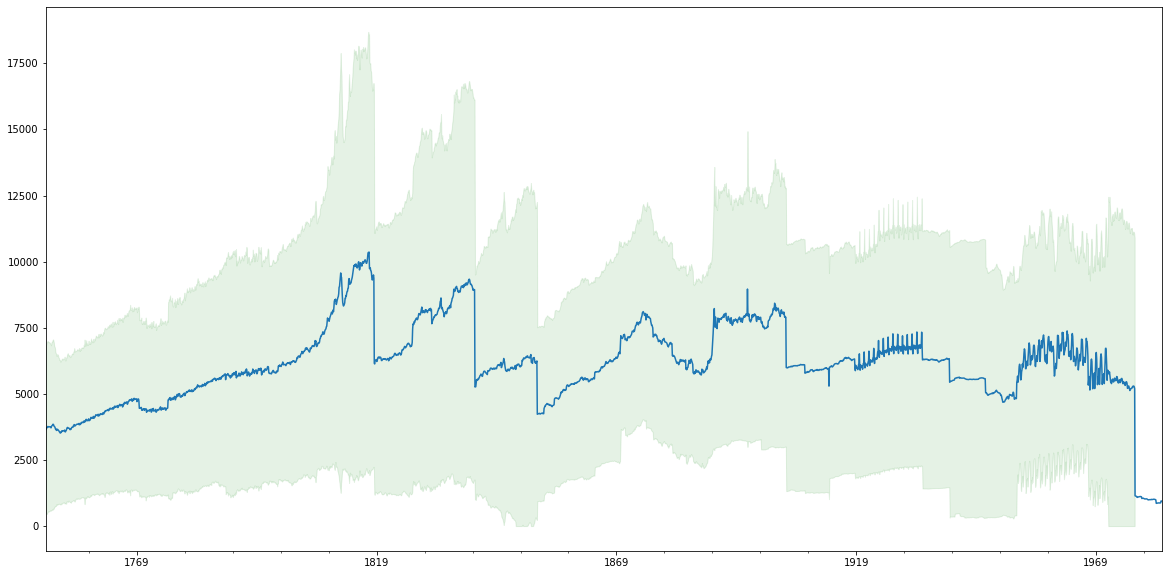
\includegraphics[width=\linewidth]{4_designing/figures/m4_monthly_plot.png}
      \caption{Plot over the average timeseries in the m4 monthly dataset with one standard deviation shown in green. Only positive values are shown as the dataset is non-negative.}
      \label{fig:m4_monthly_plot}
    \endminipage\hfill
\end{figure}

\begin{figure}[htb]
    \centering
    \minipage{0.4\textwidth}
        \begin{center}
            \begin{tabular}{||c | c | c | c | c |} 
                \hline
                statistic & mean & deviation & max & min\\
                \hline
                trend & 0.84 & 0.23 & 1.0 & 0.0 \\
                \hline
                seasonality & 0.32 & 0.30 & 1.0 & 0.0 \\
                \hline
                \hline
            \end{tabular}
            \caption{Strength of trend and seasonality of the m4 monthly dataset}
        \end{center}
    \endminipage\hfill
     \minipage{0.45\textwidth}
      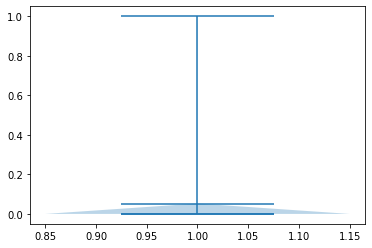
\includegraphics[width=\linewidth]{4_designing/figures/m4_monthly_violin.png}
      \caption{Scaled violin plot of the m4 monthly dataset.}
      \label{fig:m4_monthly_violin}
    \endminipage\hfill
\end{figure}

\clearpage
\subsection{M4 Quarterly}

\begin{table}[htb]
    \begin{tabular}{||c | c c c c c c c c ||} 
        \hline
       Dataset & Mean & Series & Items & Shortest & Longest & Min & Max & Frequency\\ [0.5ex] 
        \hline\hline
        train & 4141.00 & 24000 & 2214108 & 16 & 866 & 19.50 & 82210.70 & 3M\\ 
        \hline
        test & 4287.13 & 24000 & 2406108 & 24 & 874 & 19.50 & 82210.70 & 3M\\
        \hline
    \end{tabular}
    \caption{Statistics of the M4 Quarterly dataset}
\end{table}

\begin{figure}[htb]
    \centering
    \minipage{1.0\textwidth}
      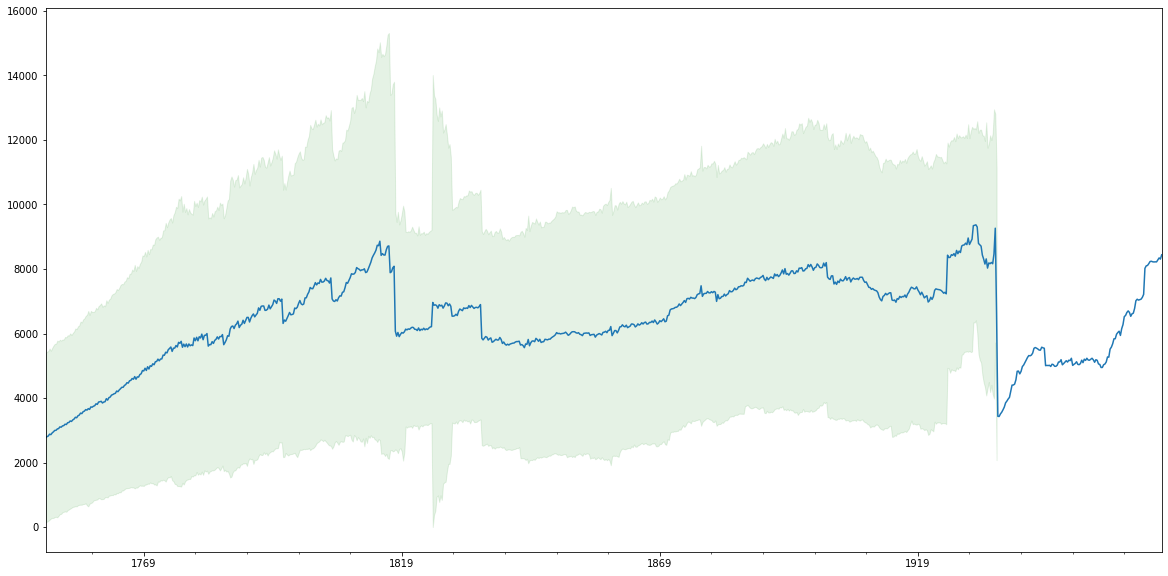
\includegraphics[width=\linewidth]{4_designing/figures/m4_quarterly_plot.png}
      \caption{Plot over the average timeseries in the m4 quarterly dataset with one standard deviation shown in green. Only positive values are shown as the dataset is non-negative.}
      \label{fig:m4_quarterly_plot}
    \endminipage\hfill
\end{figure}

\begin{figure}[htb]
    \centering
    \minipage{0.4\textwidth}
        \begin{center}
            \begin{tabular}{||c | c | c | c | c |} 
                \hline
                statistic & mean & deviation & max & min\\
                \hline
                trend & 0.90 & 0.16 & 1.0 & 0.0 \\
                \hline
                seasonality & 0.20 & 0.27 & 1.0 & 0.0 \\
                \hline
                \hline
            \end{tabular}
            \caption{Strength of trend and seasonality of the m4 quarterly dataset}
        \end{center}
    \endminipage\hfill
     \minipage{0.45\textwidth}
      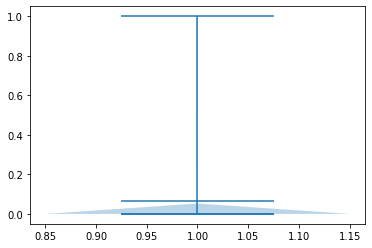
\includegraphics[width=\linewidth]{4_designing/figures/m4_quarterly_violin.png}
      \caption{Scaled violin plot of the m4 quarterly dataset.}
      \label{fig:m4_quarterly_violin}
    \endminipage\hfill
\end{figure}

\clearpage
\subsection{M4 Yearly}
\begin{table}[htb]
    \begin{tabular}{||c | c c c c c c c c ||} 
        \hline
       Dataset & Mean & Series & Items & Shortest & Longest & Min & Max & Frequency\\ [0.5ex] 
        \hline\hline
        train & 3630.52 & 23000 & 715065 & 13 & 300 & 22.10 & 115642.00 & 12M\\ 
        \hline
        test & 4076.24 & 23000 & 852909 & 19 & 300 & 22.00 & 158430.00 & 12M\\
        \hline
    \end{tabular}
    \caption{Statistics of the M4 Yearly dataset}
\end{table}


\begin{figure}[htb]
    \centering
    \minipage{1.0\textwidth}
      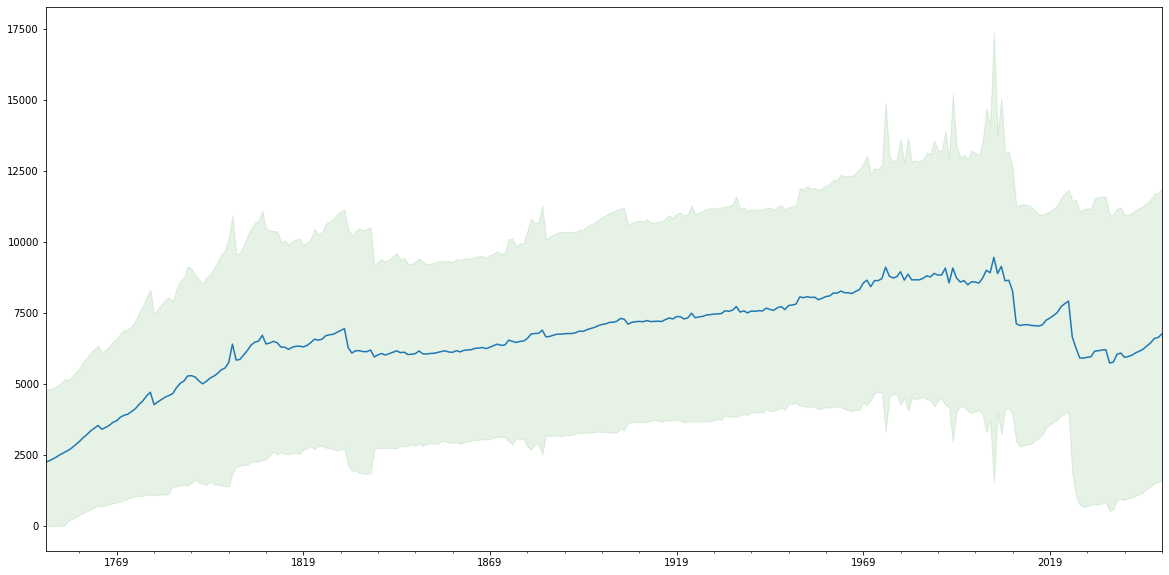
\includegraphics[width=\linewidth]{4_designing/figures/m4_yearly_plot.png}
      \caption{Plot over the average timeseries in the m4 yearly dataset with one standard deviation shown in green. Only positive values are shown as the dataset is non-negative.}
      \label{fig:m4_yearly_plot}
    \endminipage\hfill
\end{figure}

\begin{figure}[htb]
    \centering
    \minipage{0.4\textwidth}
        \begin{center}
            \begin{tabular}{||c | c | c | c | c |} 
                \hline
                statistic & mean & deviation & max & min\\
                \hline
                trend & 0.93 & 0.13 & 1.0 & 0.0 \\
                \hline
                seasonality & 0.09 & 0.16 & 0.98 & 0.0 \\
                \hline
                \hline
            \end{tabular}
            \caption{Strength of trend and seasonality of the m4 yearly dataset}
        \end{center}
    \endminipage\hfill
     \minipage{0.45\textwidth}
      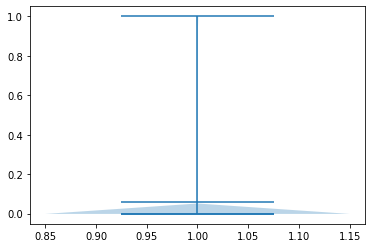
\includegraphics[width=\linewidth]{4_designing/figures/m4_yearly_violin.png}
      \caption{Scaled violin plot of the m4 yearly dataset.}
      \label{fig:m4_yearly_violin}
    \endminipage\hfill
\end{figure}


\clearpage
\subsection{M5}
\begin{table}[htb]
    \begin{tabular}{||c | c c c c c c c c ||} 
        \hline
       Dataset & Mean & Series & Items & Shortest & Longest & Min & Max & Frequency\\ [0.5ex] 
        \hline\hline
        train & 1.12 & 30490 & 57473650 & 1885 & 1885 & 0.00 & 763.00 & D\\ 
        \hline
        test & 1.13 & 30490 & 58327370 & 1913 & 1913 & 0.00 & 763.00 & D\\
        \hline
    \end{tabular}
    \caption{Statistics of the M5 dataset}
\end{table}

\begin{figure}[htb]
    \centering
    \minipage{1.0\textwidth}
      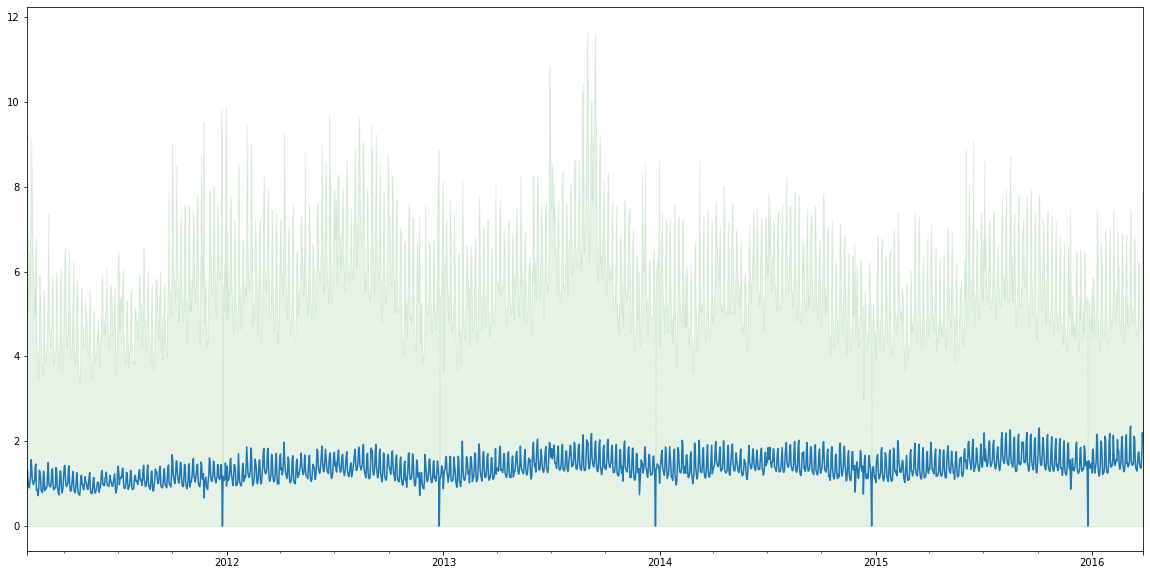
\includegraphics[width=\linewidth]{4_designing/figures/m5_plot.png}
      \caption{Plot over the average timeseries in the m5 dataset with one standard deviation shown in green. Only positive values are shown as the dataset is non-negative.}
      \label{fig:m5_plot}
    \endminipage\hfill
\end{figure}
\begin{figure}[htb]
    \centering
    \minipage{0.4\textwidth}
        \begin{center}
            \begin{tabular}{||c | c | c | c | c |} 
                \hline
                statistic & mean & deviation & max & min\\
                \hline
                trend & 0.38 & 0.32 & 1.0 & 0.0 \\
                \hline
                seasonality & 0.28 & 0.33 & 1.0 & 0.0 \\
                \hline
                \hline
            \end{tabular}
            \caption{Strength of trend and seasonality of the m5 dataset}
        \end{center}
    \endminipage\hfill
     \minipage{0.45\textwidth}
      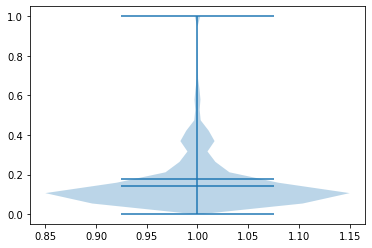
\includegraphics[width=\linewidth]{4_designing/figures/m5_violin.png}
      \caption{Scaled violin plot of the m5 dataset.}
      \label{fig:m5_violin}
    \endminipage\hfill
\end{figure}

\end{appendices}

\end{document}
